% LaTeX file for Chapter 06




\chapter{Appendix}


% - inlcude Example of ITE simulation with tram dags with complex shift: $theta + LS(X2) + CS(T, X1)$ to show how tram dags can model interactions. Maybe just refer in the methods for the CS of tram dags, or alternatively in the ITE with tram dags (where i used CI, but to show that CS is also possible to allow for specific interactions)

% Complex shift (Interaction example) to show what is also possible:
% 
% Here I just want to make a short input from another example. So there the true model was that of a logistic regression with the binary outcome Y and 3 predictors. The binary treatment T and the two continuous predictors X1 and X2. There was also an interaction effect assumed between treatment and X1. So this basically means that the effect of X1 on the outcome is different for the two treatment groups.
% And here we can show that our TRAM-DAG specified by a complex shift of T and X1 can also capture this interaction effect quite well.






\section{Interpretation of linear coefficients} \label{sec:interpretation_linear_coefficients}

The transformation model framework allows for interpretation of the coefficients in the linear shift component. The choice of the inverse-link function $F_Z$ determines the interpretation of the coefficients. For example, if the standard logistic distribution is chosen as the latent scale, i.e. $F_Z(z) = \operatorname{expit}(z)$, the coefficients can be interpreted as log-odds ratios. For $F_Z(z) = 1-\exp(-\exp(z))$, the interpretation of the coefficients changes to log-hazard ratios.

Consider the conditional transformation model:

\begin{equation}
F_{X_2 \mid X_1}(x_2) = \operatorname{expit}( h(x_2) + \beta_{12} x_1 ),
\end{equation}


where $h(x_2)$ is a smooth, monotonic transformation (e.g., a Bernstein polynomial), and $\beta_{12}$ is the coefficient representing the effect of $X_1$ on $X_2$.

Applying the logit link ($\operatorname{expit}^{-1}$) yields:

\begin{equation}
\log\left( \frac{F_{X_2 \mid X_1}(x_2)}{1 - F_{X_2 \mid X_1}(x_2)} \right)
= h(x_2) + \beta_{12} x_1.
\end{equation}


This shows that on the log-odds scale, $X_1$ has an additive linear effect on $X_2$. The corresponding odds ratio when increasing $x_1$ by one unit is:

\begin{equation}
\text{OR}_{x_1 \to x_1 + 1} = 
\frac{\exp(h(x_2) + \beta_{12}(x_1 + 1))}{\exp(h(x_2) + \beta_{12} x_1)} 
= \exp(\beta_{12}).
\end{equation}

Therefore, $\exp(\beta_{12})$ represents the multiplicative change in odds of $X_2 \le x_2$ for a one-unit increase in $X_1$, holding all else constant. This means that $\beta_{12}$ can be interpreted as a log-odds ratio.






\section{Bernstein polynomial for continuous outcomes} \label{sec:bernstein_polynomial}

In deep TRAMs, the intercept for a continuous outcome $y$ is modeled as a smooth and monotonically increasing function using a Bernstein polynomial of order $M$. Here, we focus on the more general case, where the intercept depends on the predictors $\mathbf{x}$. The same logic also applies to the simple intercept case without dependence on covariates.

The intercept of the transformation function can be written as:

\begin{equation}
h_I(y \mid \mathbf{x}) = \sum_{k=0}^{M} \vartheta_k(\mathbf{x}) \cdot B_{k, M}(s(y)),
\label{eq:bernstein_intercept}
\end{equation}

where $s(y) \in [0, 1]$ is a scaled version of the outcome $y$, and $B_{k, M}(s(y))$ denotes the $k$-th Bernstein basis polynomial of degree $M$, defined as:

\[
B_{k, M}(s(y)) = \binom{M}{k} s(y)^k (1 - s(y))^{M - k}.
\]

The parameters $\vartheta_k(\mathbf{x})$ depend on the predictors and determine the shape of the intercept function. To ensure that $h_I(y \mid \mathbf{x})$ is monotonically increasing in $y$, the coefficients must satisfy:

\[
\vartheta_0(\mathbf{x}) \leq \vartheta_1(\mathbf{x}) \leq \dots \leq \vartheta_M(\mathbf{x}).
\]

To ensure monotonicity, the unbounded parameters $\hat{\vartheta}_k(\mathbf{x}) \in \mathbb{R}$ are first predicted (by the neural network) and then transformed using a cumulative sum of softplus-transformed values. This guarantees that the resulting coefficients are non-decreasing, and therefore that the transformation function $h_I(y \mid \mathbf{x})$ is smooth and strictly monotonically increasing in $y$.
Bernstein polynomials can approximate a wide range of smooth functions, provided the degree $M$ is sufficiently large.



\subsection{Scaling and extrapolation of the Bernstein polynomial}

Because the Bernstein polynomial is only defined on the range $[0, 1]$, the outcome variable $y$ must be scaled to the unit interval. For parameter estimation alone, this scaling would be sufficient. However, the transformation function $h(y \mid \mathbf{x})$ must also be evaluable at arbitrary values of $y$, particularly those outside the range of the training data. This is essential, for instance, when performing generative sampling, where predicted outcomes may lie beyond the originally observed range of $y$.

To address this, we extend the Bernstein polynomial with a linear extrapolation in the tails. Specifically, we construct the core transformation within the 5\% and 95\% quantiles of the training outcome $y$ using the smooth Bernstein polynomial in Equation~\ref{eq:bernstein_intercept}, and extrapolate beyond this range linearly using the boundary derivatives. This results in a piecewise-defined transformation that is smooth, differentiable, strictly monotonic, and defined for all real-valued outcomes.

Let $q_{0.05}$ and $q_{0.95}$ denote the 5th and 95th empirical quantiles of $y$, computed on the training set. The scaled outcome is defined as:

\begin{equation}
s(y) = \frac{y - q_{0.05}}{q_{0.95} - q_{0.05}}.
\end{equation}

This transformation maps the central interval $[q_{0.05}, q_{0.95}]$ onto the unit interval $[0, 1]$, the domain of the Bernstein basis polynomials. Let $h_I(s(y) \mid \mathbf{x})$ be the core transformation function as defined in Equation~\eqref{eq:bernstein_intercept}. The extrapolated transformation $\tilde{h}_I(y \mid \mathbf{x})$ is then defined as:

\begin{equation}
\tilde{h}_I(y \mid \mathbf{x}) =
\begin{cases}
h_I(0 \mid \mathbf{x}) + h_I'(0 \mid \mathbf{x}) \cdot (s(y) - 0), & \text{if } s(y) < 0 \\
h_I(s(y) \mid \mathbf{x}), & \text{if } 0 \leq s(y) \leq 1 \\
h_I(1 \mid \mathbf{x}) + h_I'(1 \mid \mathbf{x}) \cdot (s(y) - 1), & \text{if } s(y) > 1
\end{cases}
\label{eq:extended_bernstein}
\end{equation}

The derivatives $h_I'(0 \mid \mathbf{x})$ and $h_I'(1 \mid \mathbf{x})$ are computed analytically from the Bernstein basis and the learned coefficients $\vartheta_k(\mathbf{x})$, ensuring smooth and differentiable transitions at the boundaries (see Section~\ref{sec:analytical_derivative_bernstein}).

This construction ensures several desirable properties. First, the transformation function $\tilde{h}_I(y \mid \mathbf{x})$ is globally defined on $\mathbb{R}$, avoiding undefined regions or discontinuities. Second, monotonicity is guaranteed due to the softplus parameterization of the coefficients $\vartheta_k(\mathbf{x})$.




\subsection{Analytical derivative of the Bernstein polynomial} \label{sec:analytical_derivative_bernstein}

To compute gradients and ensure differentiability at the extrapolation boundaries, we derive the analytical form of the derivative of the intercept of the transformation function.

Recall the general form of the intercept of the transformation function:

\begin{equation}
h_I(y \mid \mathbf{x}) = \sum_{k=0}^{M} \vartheta_k(\mathbf{x}) \cdot B_{k, M}(s(y)),
\end{equation}

where $s(y) \in [0, 1]$ is the scaled outcome, $\vartheta_k(\mathbf{x})$ are the (monotonized) coefficients, and $B_{k, M}(s(y))$ are the Bernstein basis polynomials of degree $M$.

To compute the derivative with respect to $y$, we apply the chain rule:

\begin{equation}
\frac{d}{dy} h_I(y \mid \mathbf{x}) = \sum_{k=0}^{M} \vartheta_k(\mathbf{x}) \cdot \frac{d}{dy} B_{k, M}(s(y)) = \sum_{k=0}^{M} \vartheta_k(\mathbf{x}) \cdot \frac{dB_{k, M}(s)}{ds} \cdot \frac{ds}{dy}.
\end{equation}


Since $s(y) = \frac{y - q_{0.05}}{q_{0.95} - q_{0.05}}$, its derivative is:

\begin{equation}
\frac{ds}{dy} = \frac{1}{q_{0.95} - q_{0.05}}.
\end{equation}

The derivative of the Bernstein basis polynomial is:

\begin{equation}
\frac{d}{ds} B_{k, M}(s) = M \left[ B_{k - 1, M - 1}(s) - B_{k, M - 1}(s) \right].
\end{equation}


Therefore, the full derivative is:

\begin{equation}
\frac{d}{dy} h_I(y \mid \mathbf{x}) = \frac{M}{q_{0.95} - q_{0.05}} \sum_{k=0}^{M} \vartheta_k(\mathbf{x}) \left[ B_{k - 1, M - 1}(s(y)) - B_{k, M - 1}(s(y)) \right].
\end{equation}

This expression is used to evaluate the slope of the transformation function at the borders and is also critical when computing the likelihood.





\section{Negative log-likelihood} \label{sec:nll}

\subsection{Continuous Outcome}

For a continuous outcome $Y$, the conditional cumulative distribution function (CDF) is given by:

\begin{equation}
F_{Y \mid \mathbf{X} = \mathbf{x}}(y) = F_Z(h(s(y) \mid \mathbf{x})),
\end{equation}

where $F_Z$ is the CDF of the standard logistic distribution:

\begin{equation}
F_Z(z) = \frac{1}{1 + e^{-z}}, \quad z \in \mathbb{R},
\end{equation}

and $h$ is the conditional transformation function that maps the scaled outcome $s(y)$ to the latent (log-odds) scale.

The outcome $y$ must be scaled to the unit interval $[0, 1]$ because the Bernstein polynomial is defined on this range:

\begin{equation}
s(y) = \frac{y - \min(y)}{\max(y) - \min(y)}.
\end{equation}

To compute the conditional density, we apply the change-of-variables formula:

\begin{equation}
f_{Y \mid \mathbf{X} = \mathbf{x}}(y) = f_Z(h(s(y) \mid \mathbf{x})) \cdot h'(s(y) \mid \mathbf{x}) \cdot s'(y),
\end{equation}

where $f_Z$ is the PDF of the standard logistic distribution:

\begin{equation}
f_Z(z) = \frac{e^z}{(1 + e^z)^2}, \quad z \in \mathbb{R}.
\end{equation}

The negative log-likelihood (NLL) contribution for a single observation is then given by:

\begin{equation}
\text{NLL} = - \log f_{Y \mid \mathbf{X} = \mathbf{x}}(y).
\end{equation}

Plugging in the expressions yields:

\begin{align}
\text{NLL} &= - \log f_{Y \mid \mathbf{X} = \mathbf{x}}(y) \nonumber \\
&= -h(s(y) \mid \mathbf{x}) - 2 \log(1 + \exp(-h(s(y) \mid \mathbf{x}))) \nonumber \\
&\quad + \log h'(s(y) \mid \mathbf{x}) - \log(\max(y) - \min(y)).
\end{align}


\subsection{Discrete Outcome}

For a discrete outcome (binary, ordinal, categorical) with ordered categories $y_k$, $k = 1, \ldots, K$, the transformation model defines the conditional CDF as:

\begin{equation}
F(Y \leq y_k \mid \mathbf{X} = \mathbf{x}) = F_Z(h(y_k \mid \mathbf{x})).
\end{equation}

The likelihood contribution for an observation in class $y_k$ is:

\begin{equation}
f_{Y \mid \mathbf{X} = \mathbf{x}}(y_k) =
\begin{cases}
F_Z(h(y_1 \mid \mathbf{x})), & k = 1, \\
F_Z(h(y_k \mid \mathbf{x})) - F_Z(h(y_{k-1} \mid \mathbf{x})), & k = 2, \ldots, K - 1, \\
1 - F_Z(h(y_{K-1} \mid \mathbf{x})), & k = K.
\end{cases}
\end{equation}

The corresponding NLL contribution is then:

\begin{equation}
\text{NLL} = - \log f_{Y \mid \mathbf{X} = \mathbf{x}}(y_k).
\end{equation}






\section{Encoding of discrete variables} \label{sec:encoding_discrete_variables}

In TRAM-DAGs, a variable $X_i$ can act either as a predictor variable for a child node or as an outcome variable that depends on parent nodes.

When $X_i$ is the outcome variable, and it is discrete with $K$ ordered categories (e.g., ordinal), its conditional distribution is modeled via a transformation function $h$ that defines $K-1$ cut-points. The modeling differences between continuous and discrete outcomes have already been discussed.

However, when a discrete variable $X_i$ with $K$ categories is used as a predictor variable, it should be dummy encoded. Dummy encoding creates $K - 1$ binary (0/1) indicator variables. Each binary variable corresponds to one of the non-reference categories, with the first category serving as the reference level that is not explicitly represented.

\vspace{1em}
\noindent
\textbf{Example:} Let $X$ be an ordinal variable with three levels: 1, 2, 3. Dummy encoding results in two binary variables:
\begin{itemize}
  \item $X_1$: 1 , if $X = 2$, 0 otherwise
  \item $X_2$: 1 , if $X = 3$, 0 otherwise
\end{itemize}

Now assume a continuous outcome $Y$ that depends on $X$. The transformation model is:

\[
F(Y \mid X) = F_Z(h_I(y) + x_1 \beta_1 + x_2 \beta_2)
\]

This gives us the following cases:
\begin{itemize}
  \item If $X = 1$ (reference level): $x_1 = 0$, $x_2 = 0$, so \\
  $F(Y \mid X=1) = F_Z(h_I(y))$
  \item If $X = 2$: $x_1 = 1$, $x_2 = 0$, so \\
  $F(Y \mid X=2) = F_Z(h_I(y) + \beta_1)$
  \item If $X = 3$: $x_1 = 0$, $x_2 = 1$, so \\
  $F(Y \mid X=3) = F_Z(h_I(y) + \beta_2)$
\end{itemize}

The coefficients $\beta_1$ and $\beta_2$ represent the additive shift on the latent scale (e.g., log-odds) when moving from the reference category (1) to categories 2 and 3, respectively.

Dummy encoding ensures that discrete predictors can be incorporated into the deep TRAM framework and maintain interpretability.



\section{Scaling of continuous variables} \label{sec:scaling_continuous_variables}

Neural networks work best when the input variables are standardized. 

A linear, monotonic, and invertible transformation of a predictor variable changes the interpretation of the coefficient. Scaling a predictor variable $X$ as $X_{\text{std}} = (X - \mu_X) / \sigma_X$ implies that the coefficient $\tilde{\beta}$ is interpreted as the change in log-odds for a one standard deviation increase in the predictor variable -- or equivalently, for a one unit increase in the standardized predictor. This differs from the interpretation of the original coefficient $\beta$, which represents the change in log-odds for a one-unit increase in the raw predictor variable.


In contrast, the standardization of the outcome variable does not affect the interpretation of the model, due to the scale invariance of the log-odds. Suppose we standardize the outcome $Y$ as follows:

\[
Y_{\text{std}} = \frac{Y - \mu_Y}{\sigma_Y}
\]

This transformation is linear, monotonic, and invertible:

\[
Y = Y_{\text{std}} \cdot \sigma_Y + \mu_Y
\]

Therefore, for any threshold $y$, we have the equivalence:

\[
P(Y < y \mid X) = P\left(Y_{\text{std}} < \frac{y - \mu_Y}{\sigma_Y} \mid X\right)
\]


This means, the probability of being below a particular quantile remains the same after standardization. Consequently, the interpretation of coefficients in models with a continuous outcome remains unchanged. Specifically, the log-odds ratio


\[
\log \left( \frac{P(Y < y \mid X + 1)}{1 - P(Y < y \mid X + 1)} \right) -
\log \left( \frac{P(Y < y \mid X)}{1 - P(Y < y \mid X)} \right)
\]

is equal to

\[
\log \left( \frac{P\left(Y_{\text{std}} < \frac{y - \mu_Y}{\sigma_Y} \mid X + 1\right)}{1 - P\left(Y_{\text{std}} < \frac{y - \mu_Y}{\sigma_Y} \mid X + 1\right)} \right) -
\log \left( \frac{P\left(Y_{\text{std}} < \frac{y - \mu_Y}{\sigma_Y} \mid X\right)}{1 - P\left(Y_{\text{std}} < \frac{y - \mu_Y}{\sigma_Y} \mid X\right)} \right)
\]

as long as the same quantile (i.e., probability threshold) is used. Thus, the coefficient $\beta$ reflects the same change in log-odds per one-unit increase in the (standardized) predictor, regardless of whether the outcome is standardized or not.


The general form of the transformation model is:


\[
P(Y < y \mid X = x) = F_z\left(h(Y) + \beta \cdot X\right)
\]

but now consider the case where this model is fitted using standardized outcome and predictors:

\[
P(Y_{\text{std}} < y_{\text{std}} \mid X_{\text{std}} = x_{\text{std}}) = F_z\left(\tilde{h}(Y_{\text{std}}) + \tilde{\beta} \cdot X_{\text{std}}\right)
\]


where $\tilde{h}$ and $\tilde{\beta}$ are the estimated transformation function and coefficients after standardizing the outcome and predictors.



\textbf{Example:} To evaluate the probability \( P(Y < 20 \mid X = 3) \) in the standardized setting, we use:


\[
P\left(\frac{Y - \mu_Y}{\sigma_Y} < \frac{20 - \mu_Y}{\sigma_Y} \,\middle|\, X_{\text{std}} = \frac{3 - \mu_X}{\sigma_X} \right)
= F_z\left(\tilde{h}\left(\frac{20 - \mu_Y}{\sigma_Y}\right) + \tilde{\beta} \cdot \frac{3 - \mu_X}{\sigma_X} \right)
\]


In summary, standardizing predictors changes coefficient interpretation, whereas outcome standardization does not affect interpretability or model validity.





\section{Modeling interactions with complex shift (CS)} \label{sec:complex_shift}

% file ITE_simulation_CS.R

\begin{figure}[htbp]
\centering
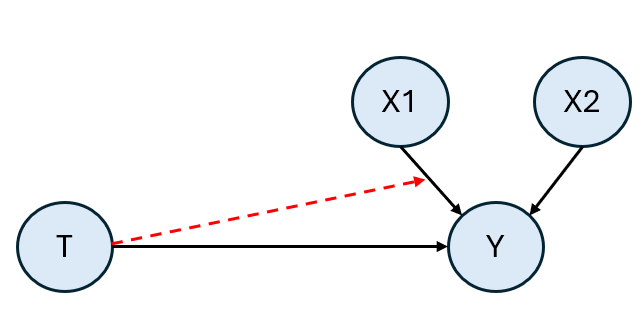
\includegraphics[width=0.4\textwidth]{img/appendix_dag_cs_interaction.png}
\caption{DAG for the complex shift example. The treatment $T$ interacts with the covariate $X_1$ to influence the outcome $Y$. The covariate $X_2$ has a direct effect on the outcome.}
\label{fig:complex_shift_dag}
\end{figure}


The aim of this section is to show how TRAM-DAGs can effectively model interactions between multiple variables in a customizable way, using either a complex shift (CS) or a complex intercept (CI). 

Here, we provide an example based on a simple DAG, as visualized in Figure~\ref{fig:complex_shift_dag}. Assume that the binary treatment $T$ is sampled from a Bernoulli distribution with probability 0.5. The covariates $X_1$ and $X_2$ represent baseline characteristics and are sampled from a standard normal distribution with a compound symmetric covariance matrix ($\rho = 0.1$). The outcome $Y$ is binary and sampled from a Bernoulli distribution with a probability that depends on the treatment $T$ and the covariates $X_1$ and $X_2$. The treatment $T$ interacts with the covariate $X_1$ to influence the outcome, while the covariate $X_2$ has a direct effect on the outcome. The formula for the outcome (on the log-odds scale) is given by:



\[
\text{logit}(P(Y=1 \mid T, X_1, X_2)) = \beta_0 + X_1 \beta_1 + X_2 \beta_2 + T \beta_3 + \textcolor{red}{T X_1\beta_4}
\]

where $\beta_0 = 0.45$, $\beta_1 = -0.5$, $\beta_2 = 0.1$, $\beta_3 = -0.85$, and $\beta_4 = 0.7$. The interaction term $T X_1$ allows the effect of $X_1$ on the outcome to vary depending on the treatment group. This results in a heterogeneous treatment effect. 
We sample 20,000 training observations from this logistic data-generating process, and model it using a TRAM-DAG following the assumed structure in the DAG in Figure~\ref{fig:complex_shift_dag}. The TRAM-DAG is specified with a complex shift (CS) of the treatment $T$ and the covariate $X_1$, which allows it to capture the interaction effect.

\[
h(Y_k \mid T, X_1, X_2) = \vartheta_k + \textcolor{red}{\text{CS}(T, X_1)} + \text{LS}(X_2)
\]

where $K = 1$ because the outcome is binary. The neural network for the CS is defined as shown in Figure~\ref{fig:complex_shift_nn}, taking the treatment $T$ and the covariate $X_1$ as inputs, which allows them to interact. 
After training the TRAM-DAG, we can visualize the resulting learned complex shift for each of the treatment groups, as illustrated in Figure~\ref{fig:CS_interaction}. Due to the interaction, the effect of the covariate $X_1$ on the outcome $Y$ differs between the treatment groups. The estimated effect aligns with the one specified in the data-generating process.


\begin{figure}[htbp]
\centering
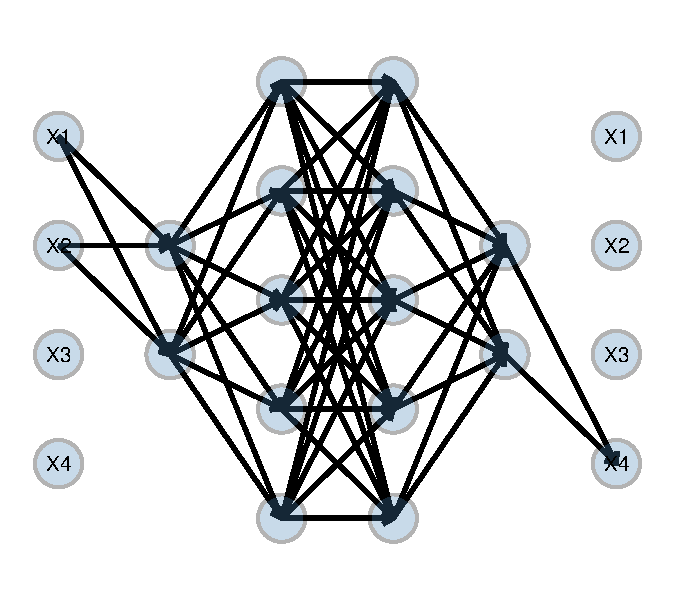
\includegraphics[width=0.5\textwidth]{img/appendix_CS_NN_interaction.pdf}
\caption{Neural network architecture for the complex shift (CS) effect of the treatment $T$ and the covariate $X_1$ on the outcome $Y$ ($X_4$). ReLU activation and batch normalization were used in the hidden layers. The deep neural network enables interactions between the input variables.}
\label{fig:complex_shift_nn}
\end{figure}


\begin{figure}[htbp]
\centering
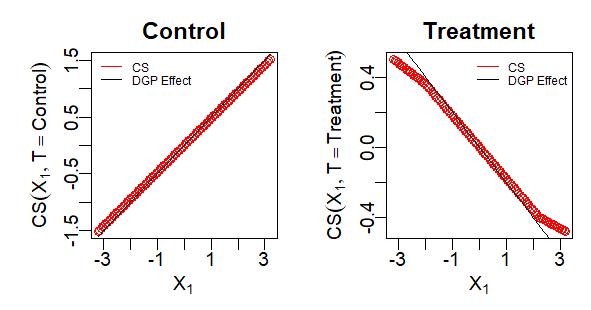
\includegraphics[width=0.75\textwidth]{img/appendix_CS_T_X1_interaction.png}
\caption{Learned complex shift (CS) effect of the treatment $T$ and the covariate $X_1$ on the outcome (log-odds scale). Left: effect of $X_1$ on the outcome $Y$ in the control group ($T=0$); Right: effect of $X_1$ on the outcome $Y$ in the treatment group ($T=1$).}
\label{fig:CS_interaction}
\end{figure}


The fitted TRAM-DAG was then used to estimate the individualized treatment effect (ITE) for each sample $i$, defined as $\text{ITE}_i(\mathbf{x}_i) = P(Y_i = 1 \mid T = 1, \mathbf{X}_i = \mathbf{x}_i) - P(Y_i = 1 \mid T = 0, \mathbf{X}_i = \mathbf{x}_i)$. We estimated the ITEs on the test set using the trained TRAM-DAG. In the uncalibrated model, the predicted ITEs did not perfectly match the true ITEs -- although the difference was only a small deviation. Therefore, we recalibrated the model by fitting a generalized additive model (GAM) on a separate calibration dataset using the predicted probabilities from the TRAM-DAG. The recalibrated ITEs aligned well with the true ITEs. The results are shown in Figure~\ref{fig:ITE_interaction}.

This example demonstrates how TRAM-DAGs can be used to model interactions, which are crucial for accurate ITE estimation when applying the model as an S-learner.


\begin{figure}[htbp]
\centering
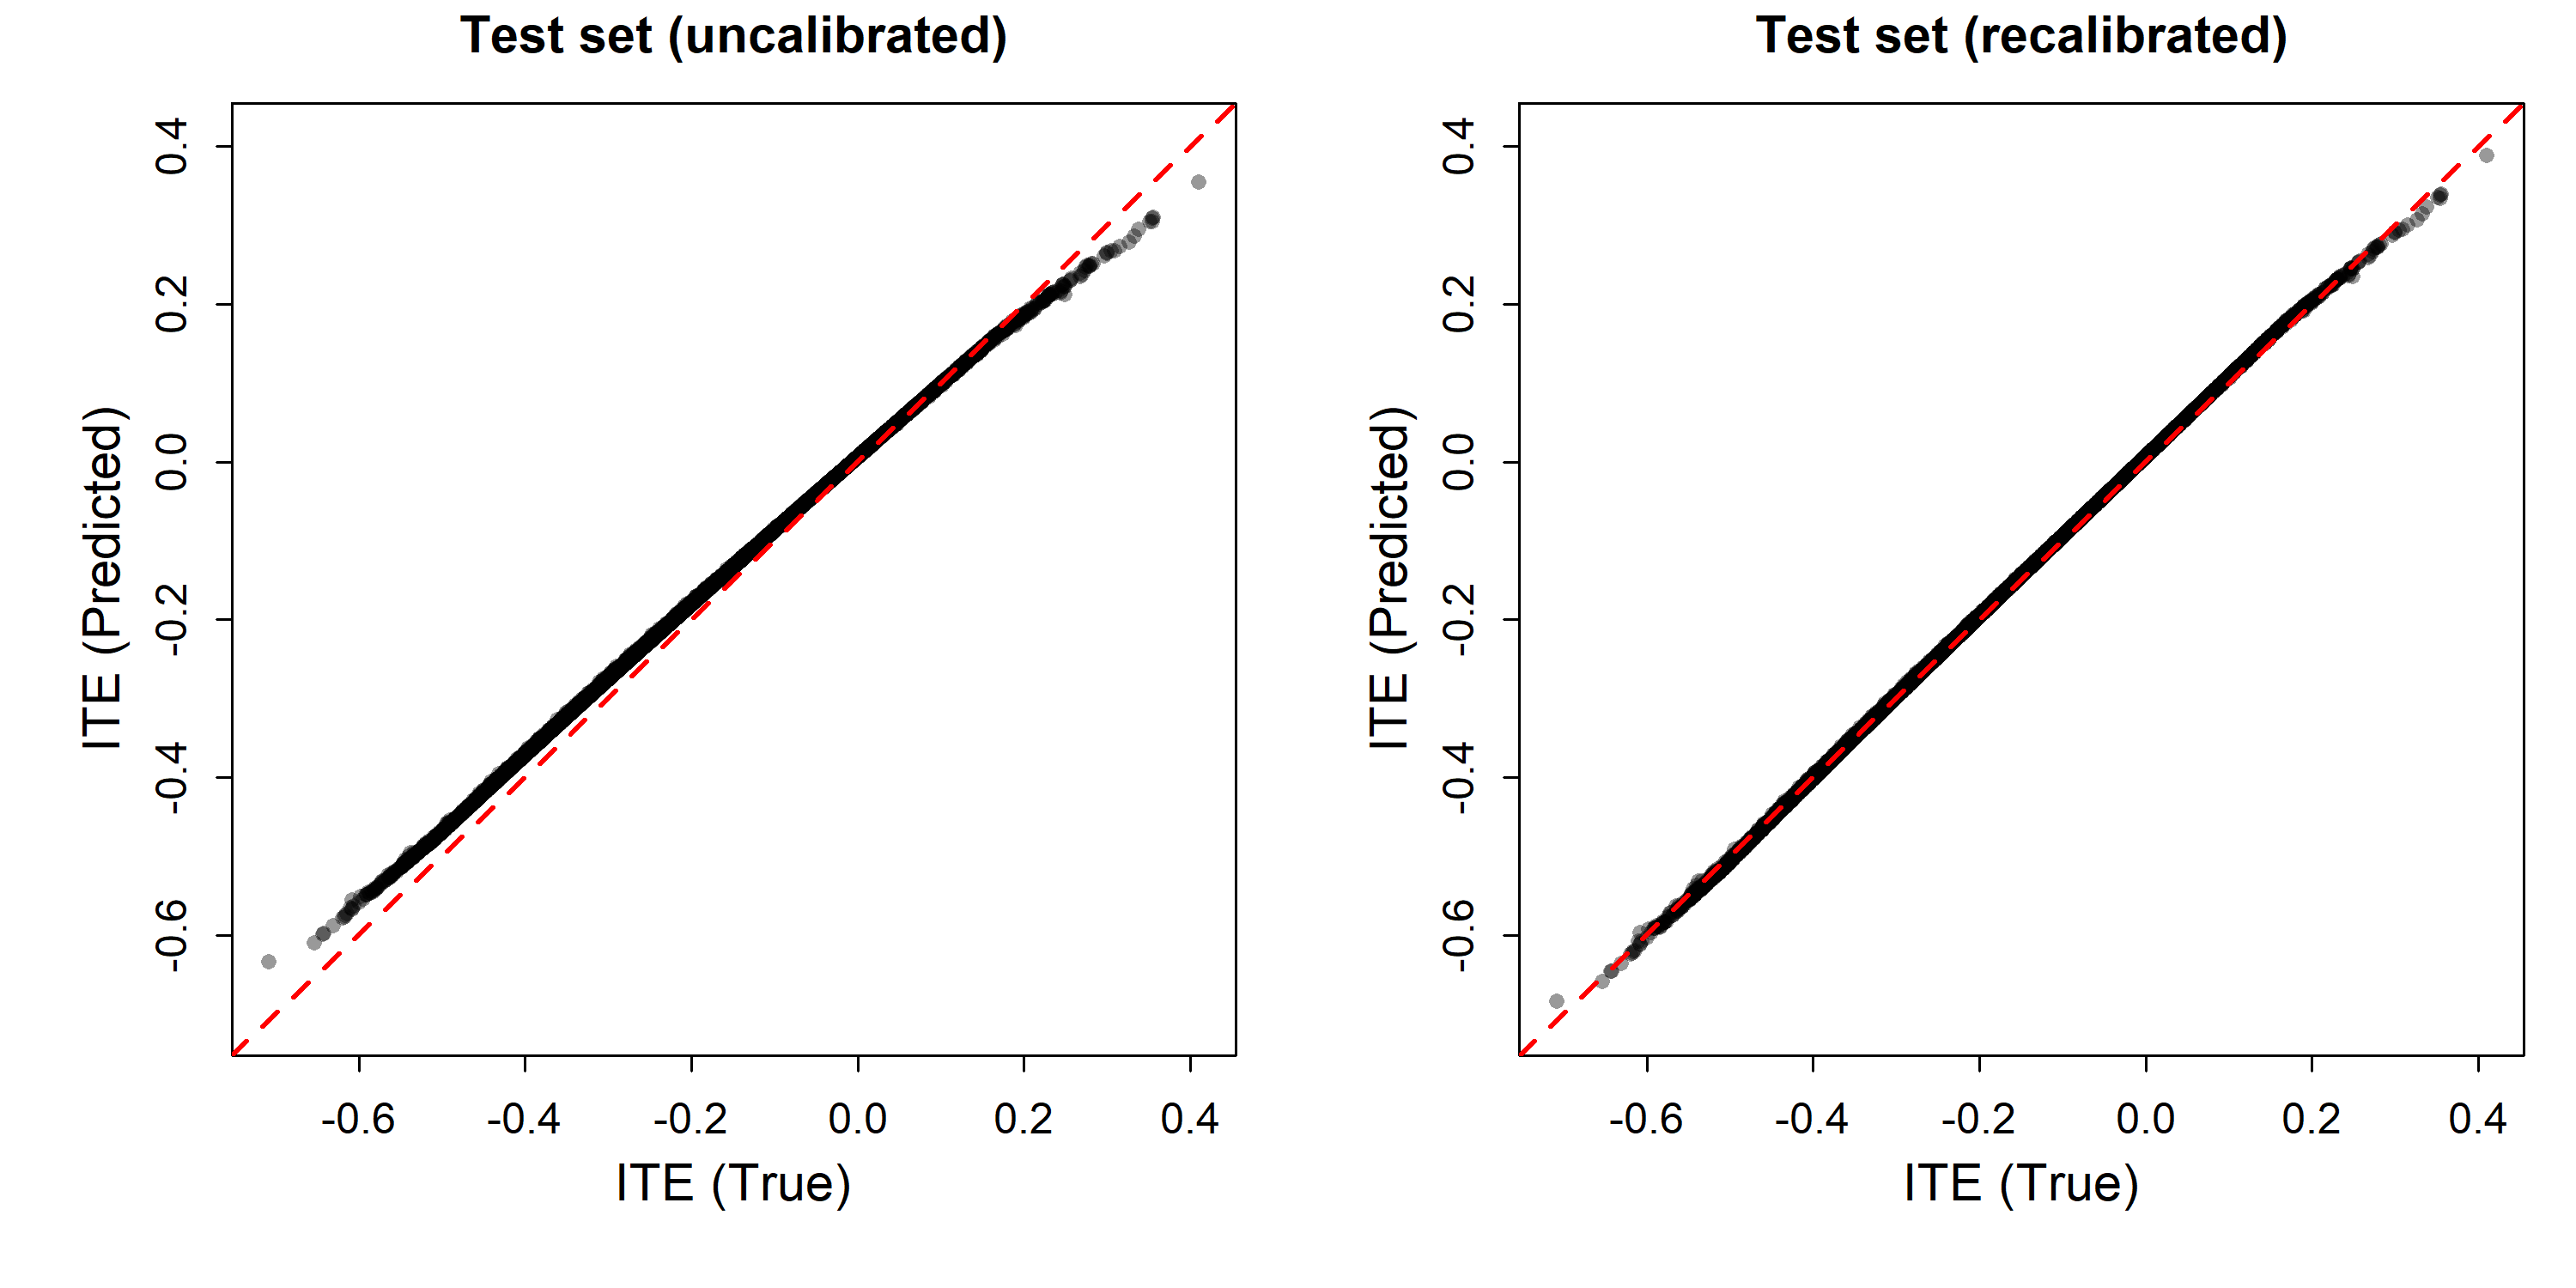
\includegraphics[width=0.75\textwidth]{img/appendix_ITE_recal.png}
\caption{Estimated individualized treatment effects (ITE) using the fitted TRAM-DAG with a complex shift (CS). Left: estimated vs. true ITEs using the uncalibrated model. Right: estimated vs. true ITEs after recalibration. Recalibration was performed using an independent calibration dataset, where a generalized additive model (GAM) was fitted to recalibrate the probability estimates produced by the TRAM-DAG.}
\label{fig:ITE_interaction}
\end{figure}



\section{Experiment 2: Calibration plots} \label{sec:calibrations_experiment2}

Figures \ref{fig:calibration_IST_glm}-\ref{fig:calibration_IST_TRAM_DAG} show the calibration plots of predicted risks versus observed outcome proportions for the models applied in Experiment 2 (International Stroke Trial, IST).


% It becomes apparent, that tuning the random forest model out-of-bag leads to a poor calibration on the training set, but due to better generalization it leads to a better calibration on the test set.

\begin{figure}[htbp]
\centering
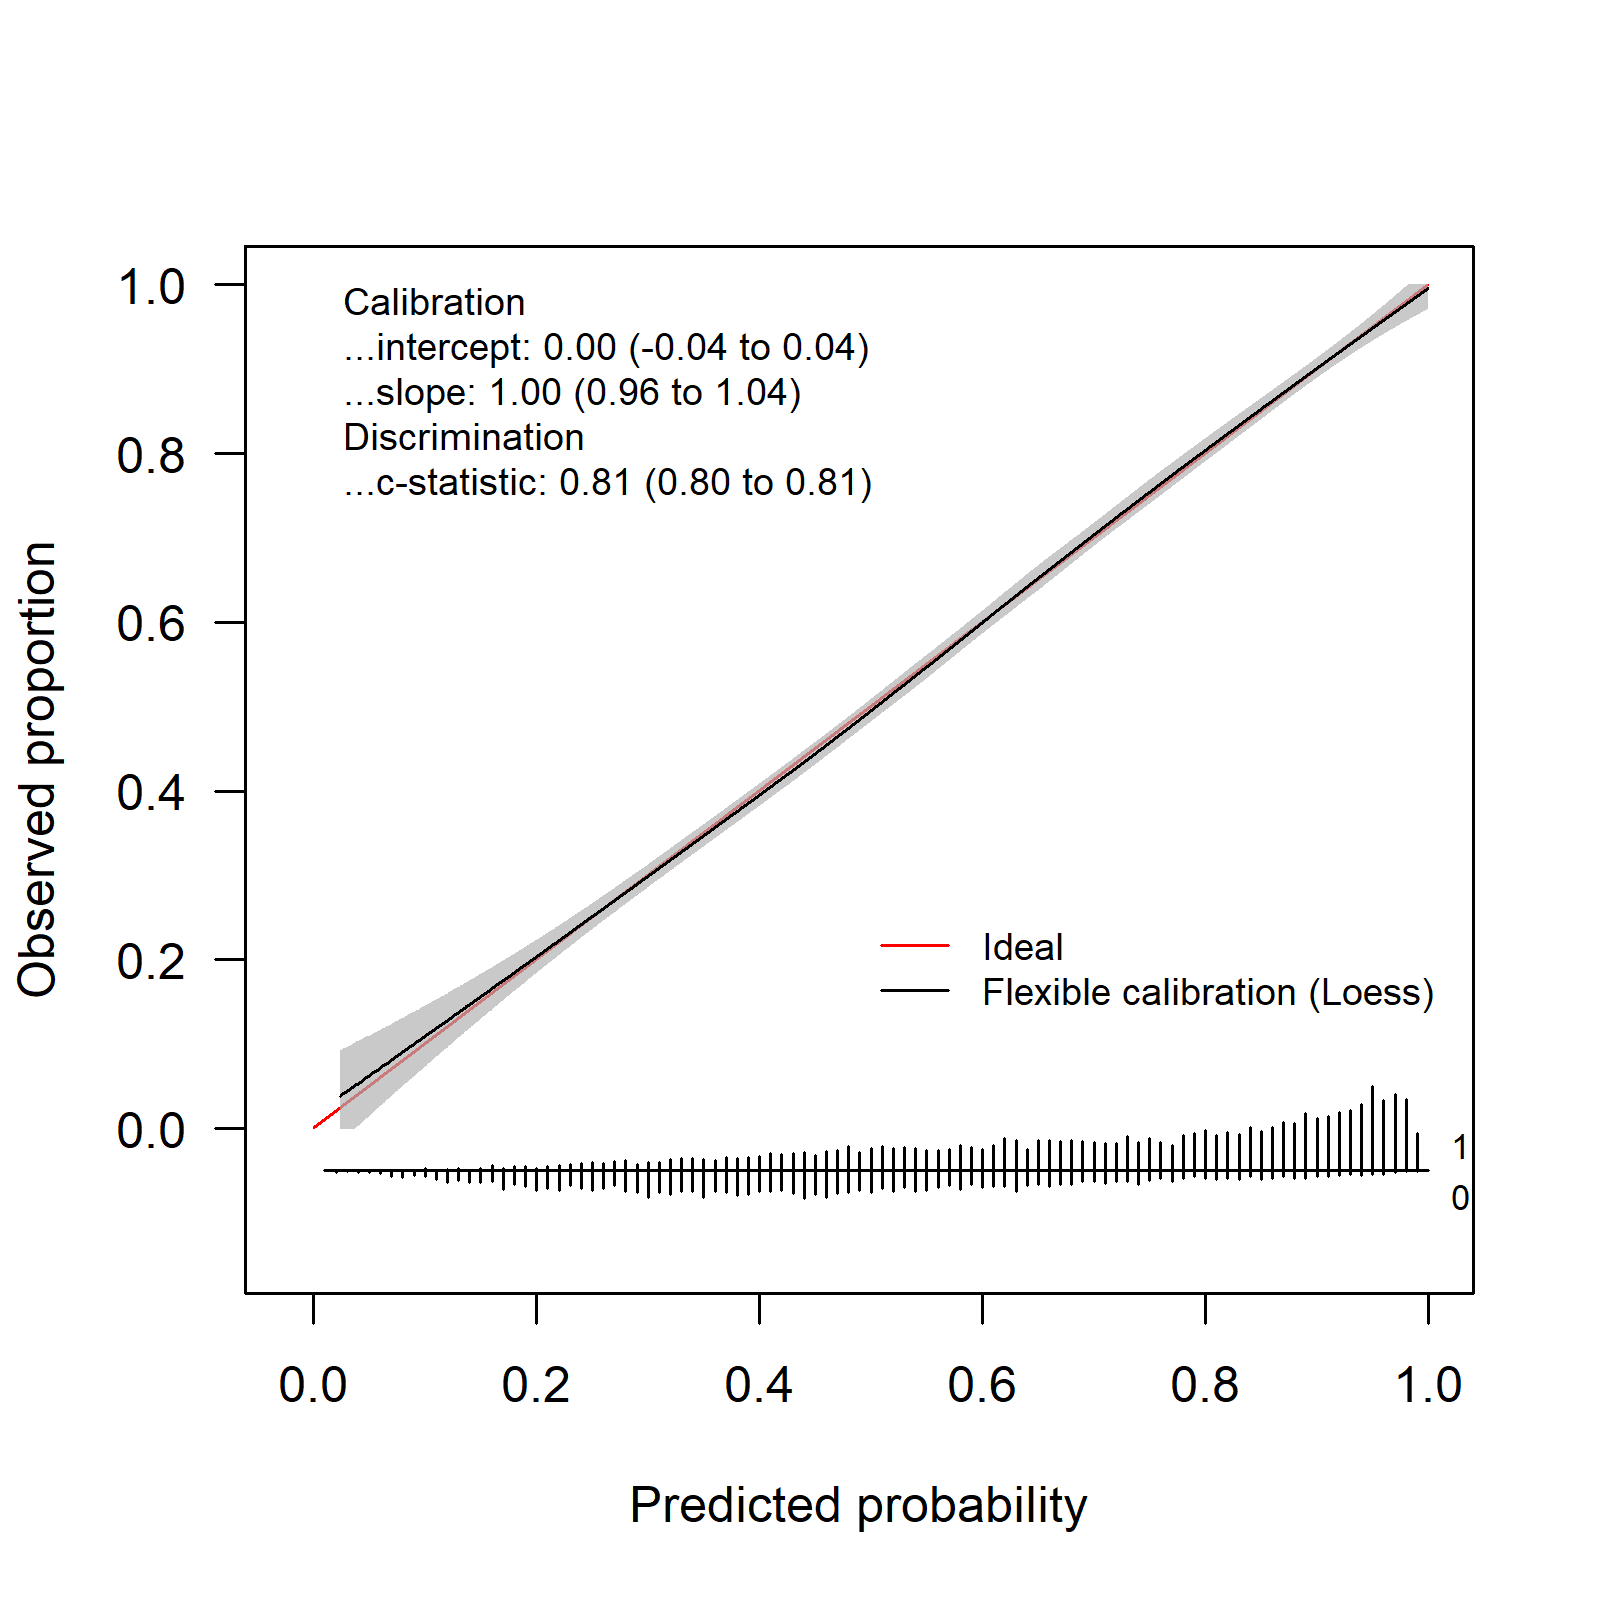
\includegraphics[width=0.45\textwidth]{img/results_IST/glm_tlearner_train_calibration_plot.png}
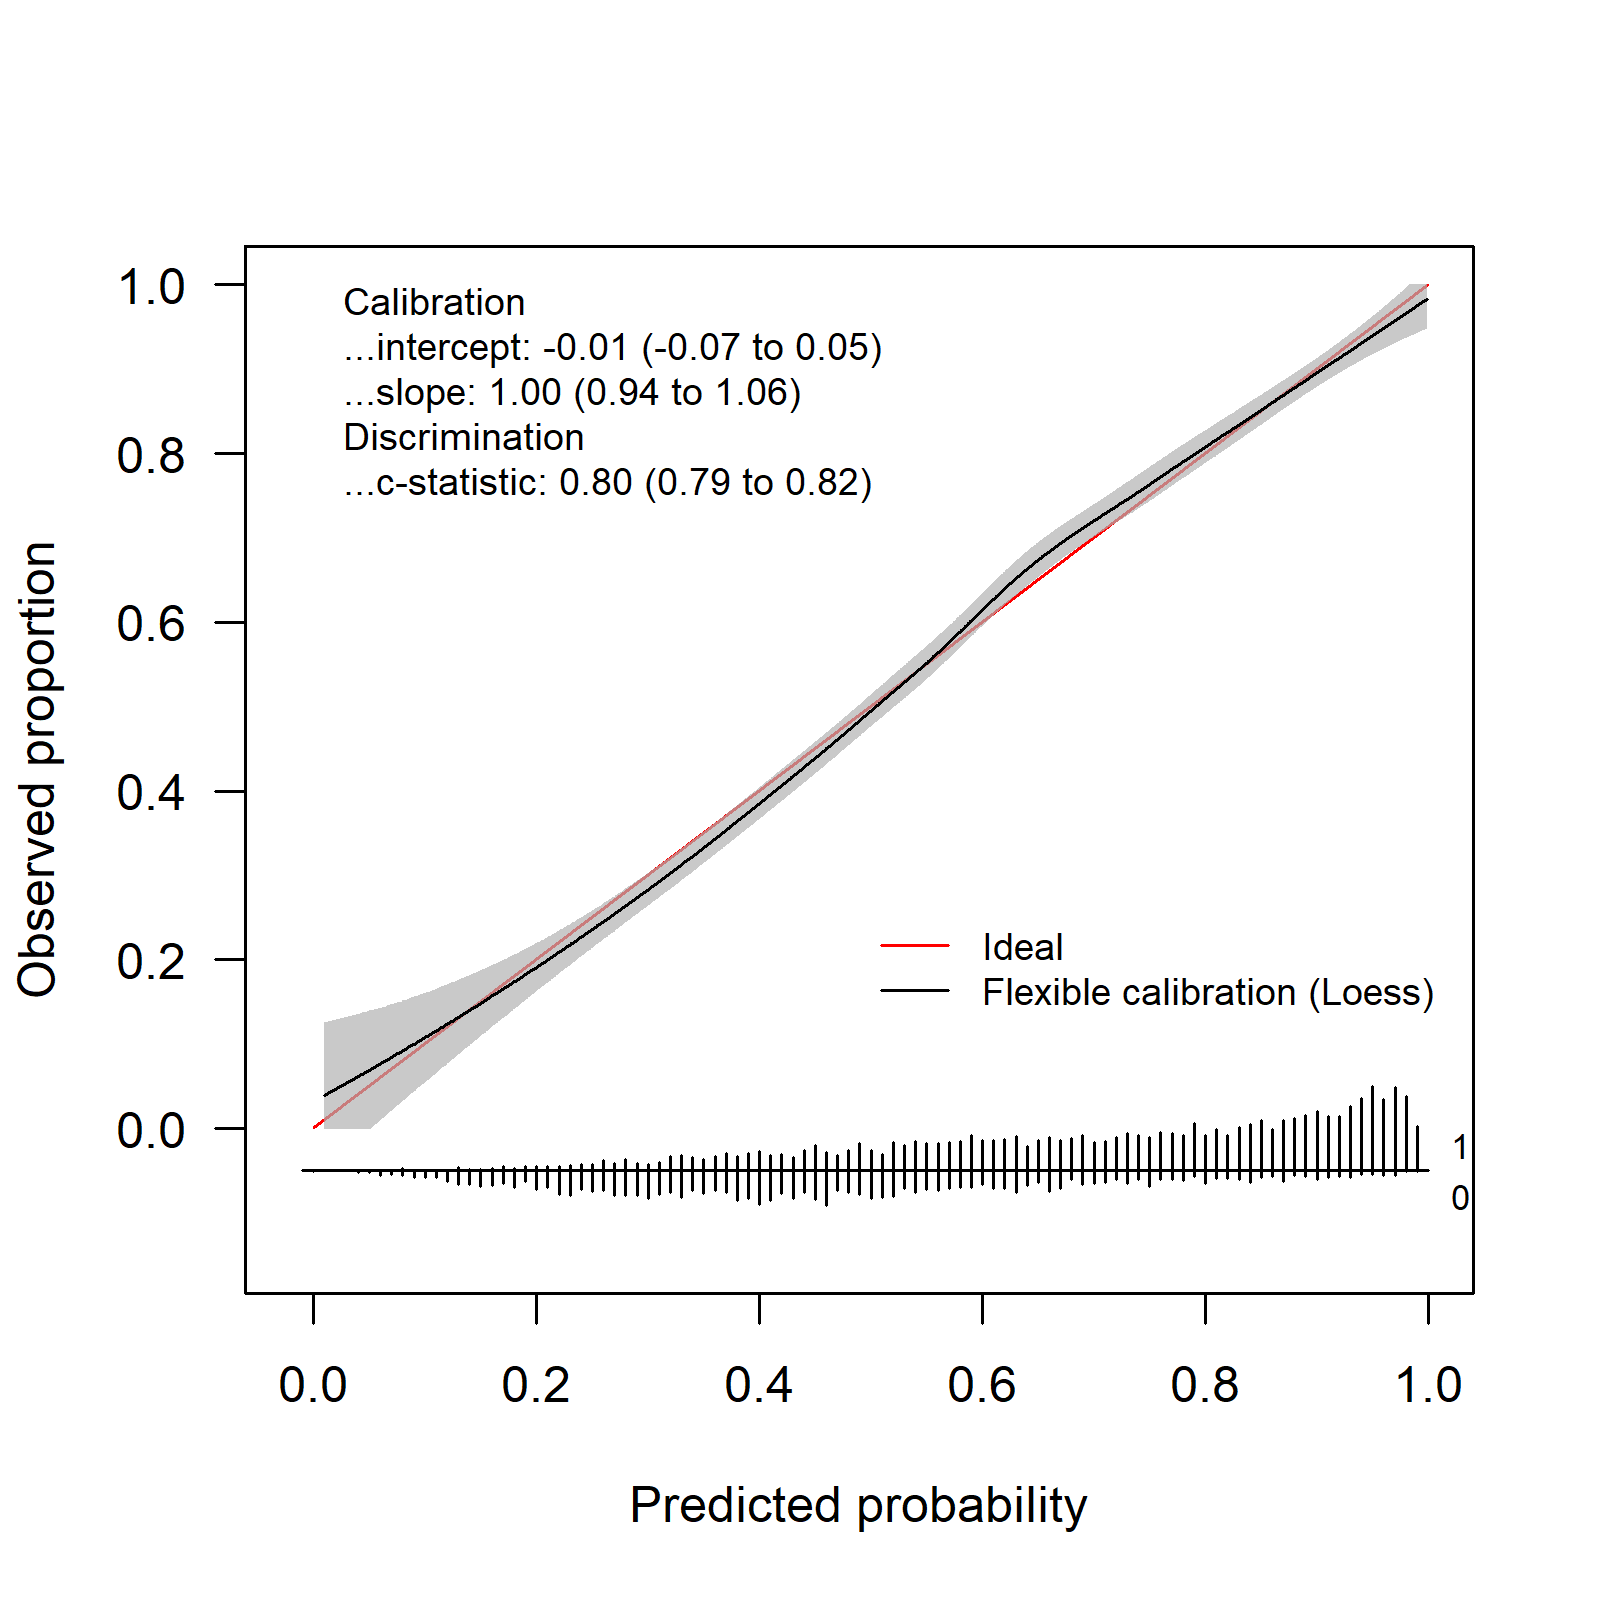
\includegraphics[width=0.45\textwidth]{img/results_IST/glm_tlearner_test_calibration_plot.png}
\caption{Calibration plot for the T-learner logistic regression applied to the International Stroke Trial (IST) in Experiment 2. The plot shows predicted risks versus observed event proportions. Left: training dataset; Right: test dataset.}
\label{fig:calibration_IST_glm}
\end{figure}


\begin{figure}[htbp]
\centering
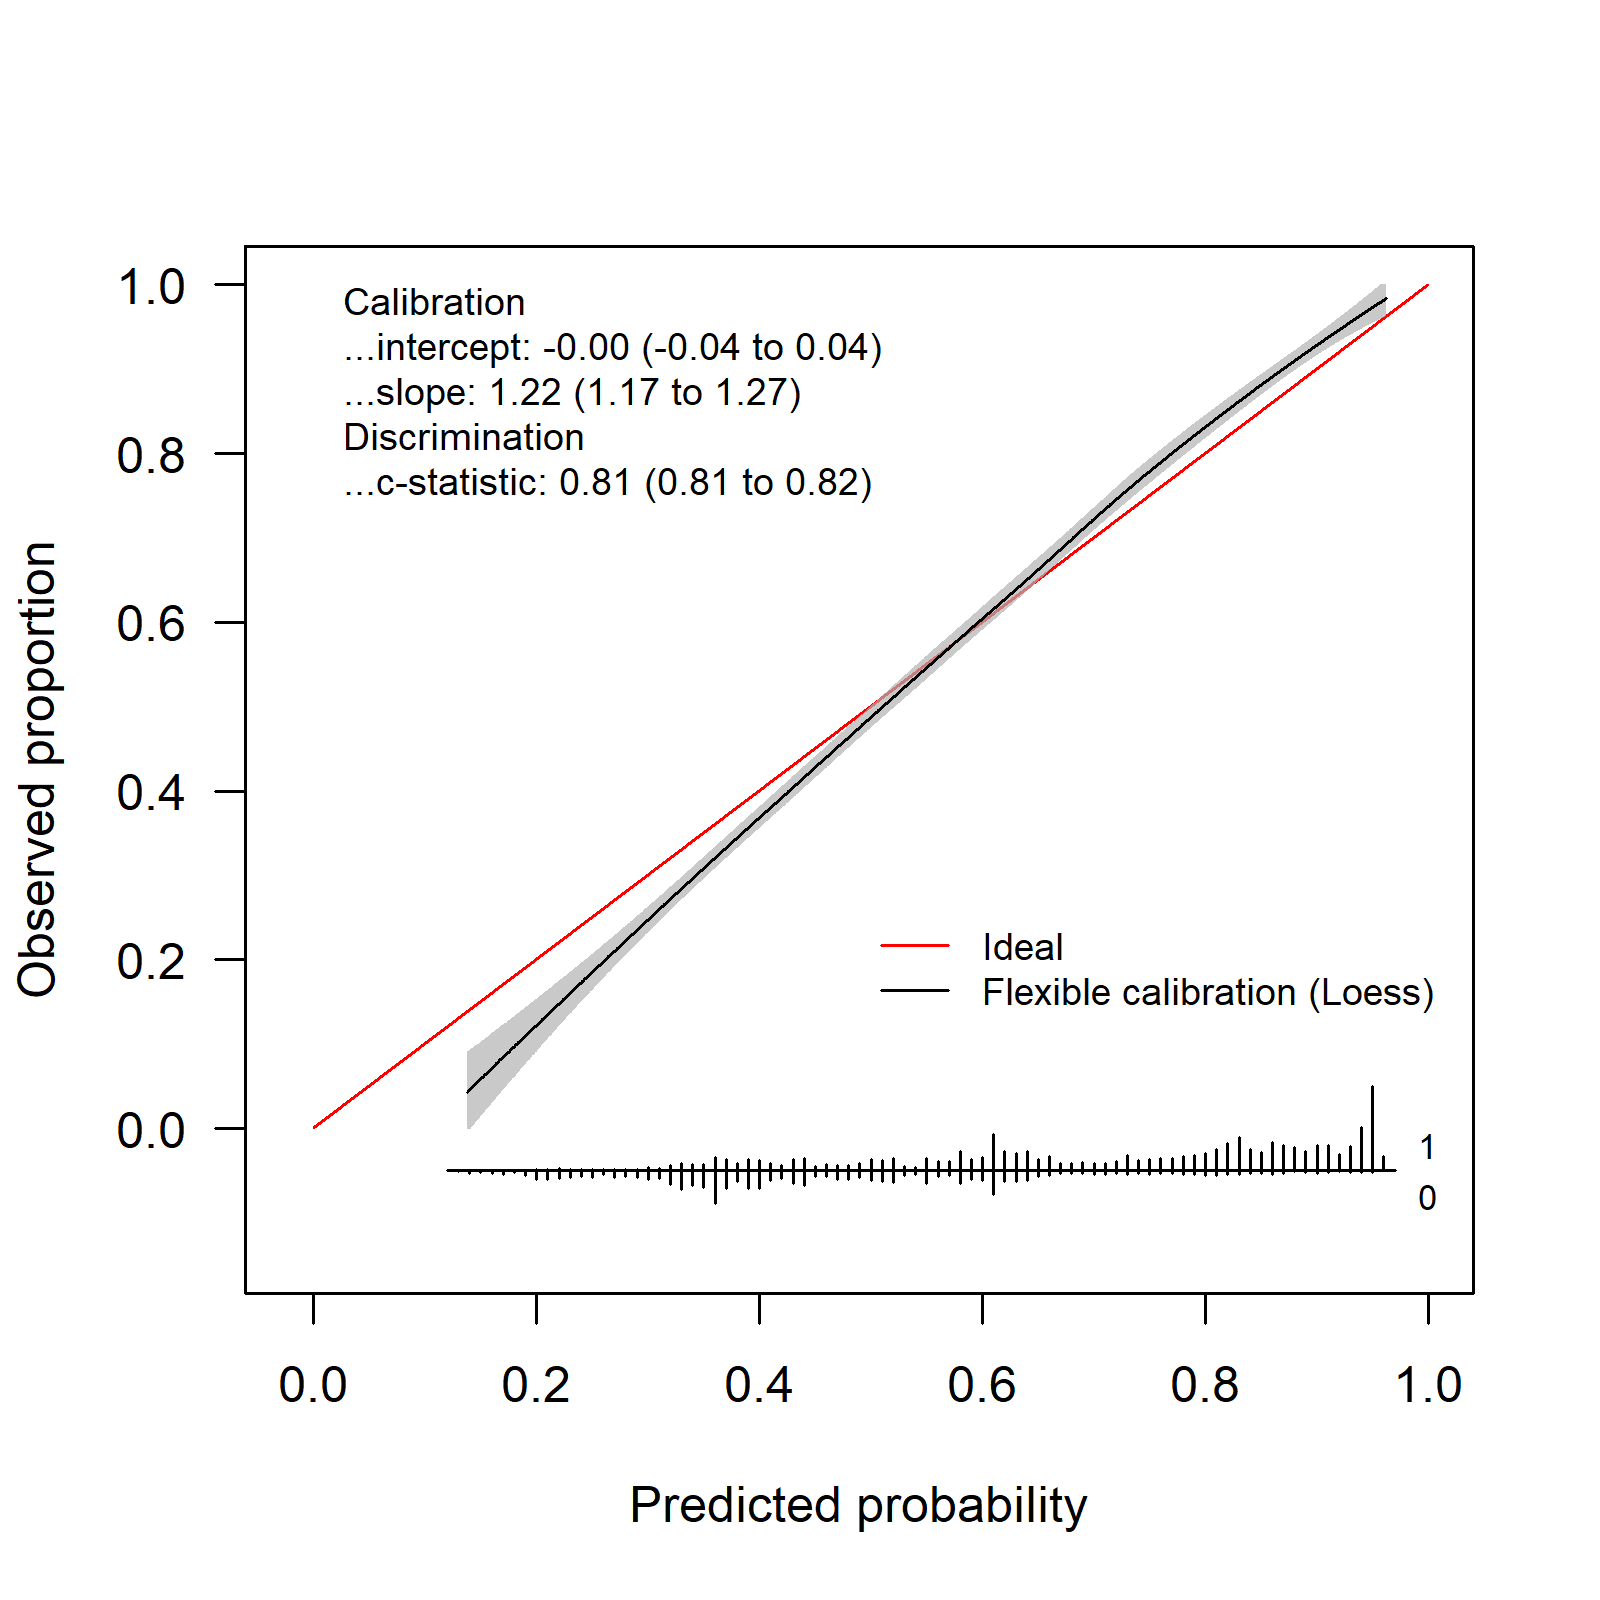
\includegraphics[width=0.45\textwidth]{img/results_IST/IST_tuned_rf_tlearner_train_calibration_plot.png}
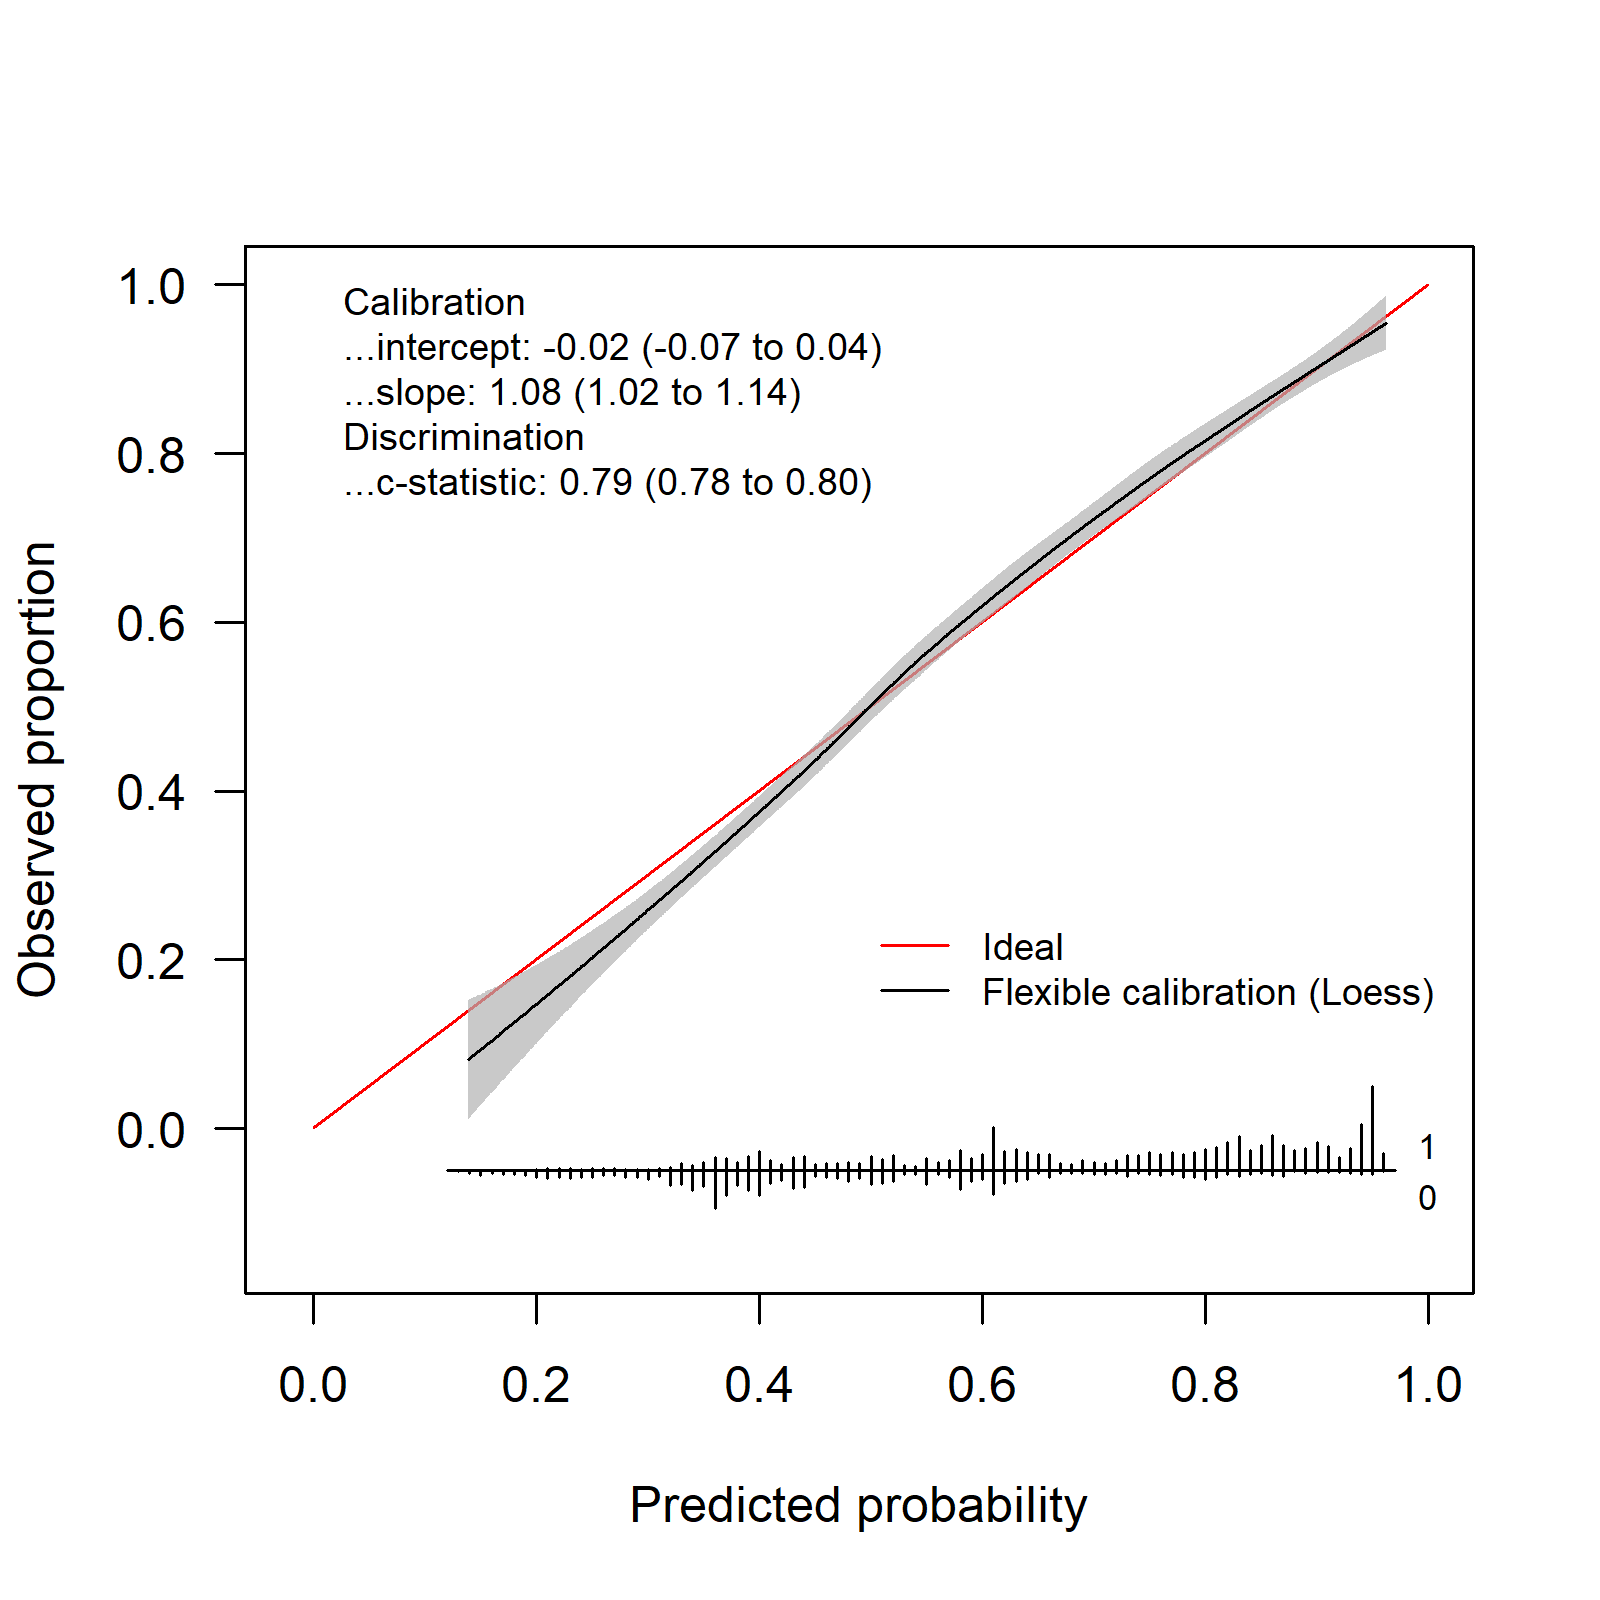
\includegraphics[width=0.45\textwidth]{img/results_IST/IST_tuned_rf_tlearner_test_calibration_plot.png}
\caption{Calibration plot for the T-learner tuned random forest applied to the International Stroke Trial (IST) in Experiment 2. The plot shows predicted risks versus observed event proportions. Left: training dataset; Right: test dataset.}
\label{fig:calibration_IST_tuned_rf}
\end{figure}


\begin{figure}[htbp]
\centering
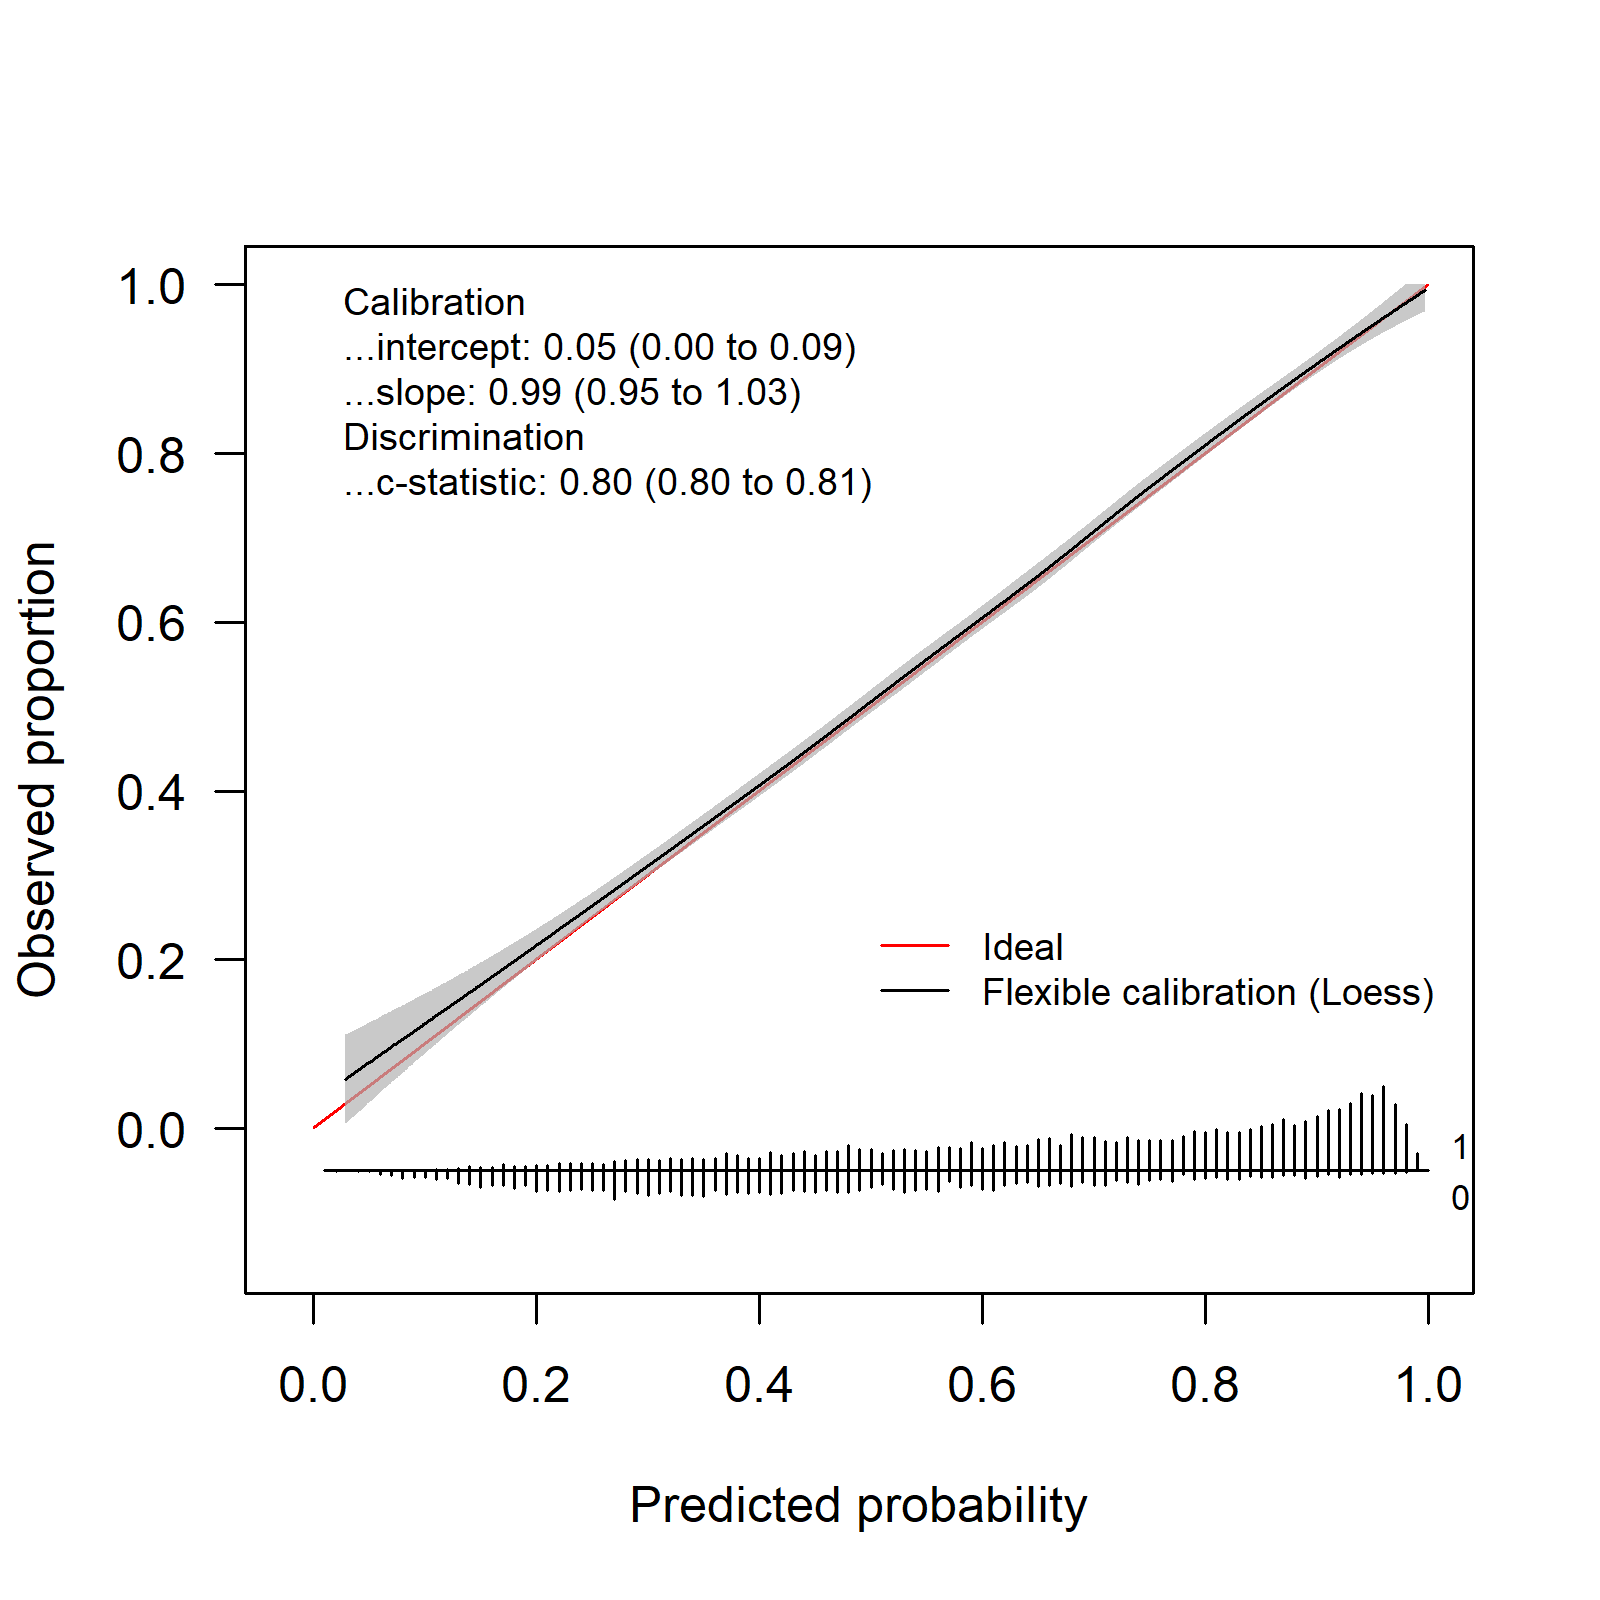
\includegraphics[width=0.45\textwidth]{img/results_IST/IST_TRAM_DAG_slearner_train_calibration_plot.png}
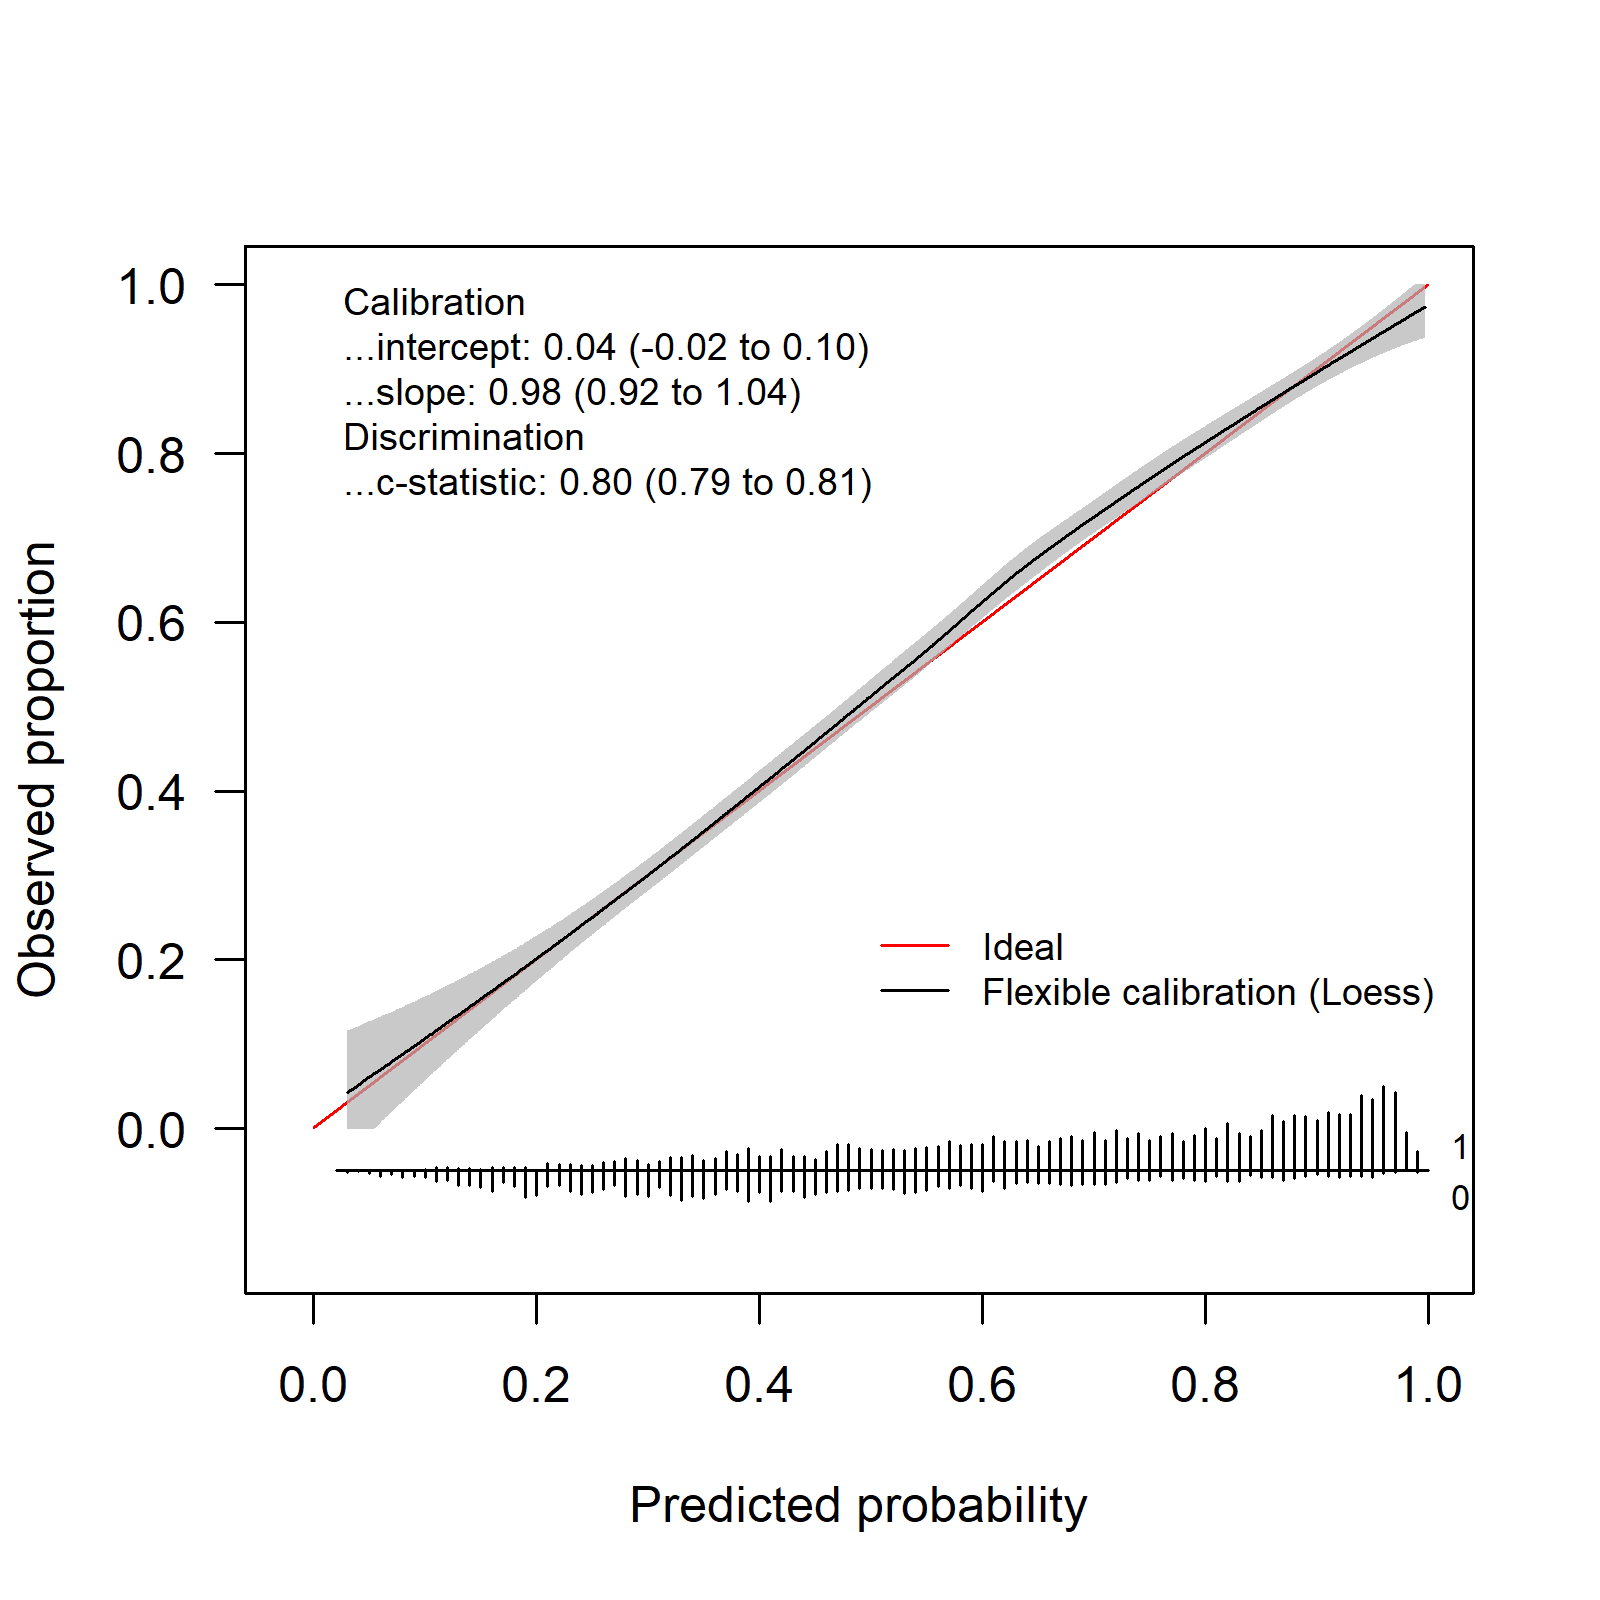
\includegraphics[width=0.45\textwidth]{img/results_IST/IST_TRAM_DAG_slearner_test_calibration_plot.png}
\caption{Calibration plot for the S-learner TRAM-DAG applied to the International Stroke Trial (IST) in Experiment 2. The plot shows predicted risks versus observed event proportions. Left: training dataset; Right: test dataset.}
\label{fig:calibration_IST_TRAM_DAG}
\end{figure}


\clearpage


\section{Experiment 3: Standard random forest for ITE estimation} \label{sec:default_rf_ite}

In Section~\ref{sec:ite_models}, we emphasized the importance of model calibration when estimating individualized treatment effects. Here, we present results from a default (untuned) random forest model in Scenario~(1), where all variables are observed and both treatment and interaction effects are strong (see Figure~\ref{fig:fully_observed_dag_rf_appendix}). The corresponding model results are shown in Figure~\ref{fig:fully_observed_glm_rf}.

In the scatterplot of true vs. predicted probabilities for $\text{P}(Y_i = 1 \mid \mathbf{X}_i = \mathbf{x}_i, T_i = t_i)$ in the training set, it is visible that the model does not predict probabilities accurately and is therefore poorly calibrated. This poor calibration also affects the estimated ITEs.

By comparison, the results of the tuned random forest (Figure~\ref{fig:fully_tuned_rf_tlearner}) show that the model is better calibrated and the estimated ITEs are close to the true ITEs. These results highlight the importance of model tuning for ITE estimation, as poor calibration can lead to biased estimates of individualized treatment effects.



\begin{figure}[htbp]
\centering
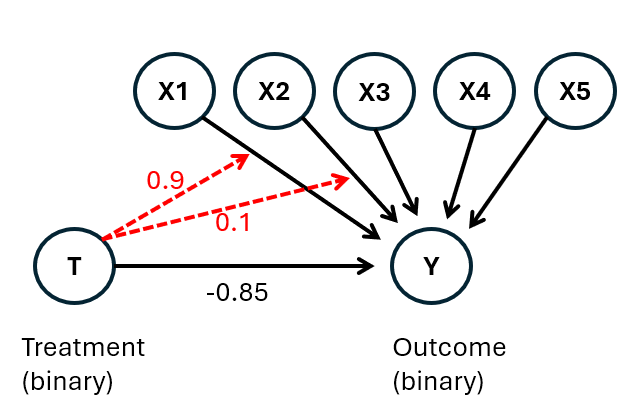
\includegraphics[width=0.35\textwidth]{img/results_ITE_simulation/simulation_observed.png}
\caption{DAG for Scenario~(1), where all variables are observed and both treatment and interaction effects are strong. The numbers indicate the coefficients on the log-odds scale. Red arrows represent interaction effects between treatment ($T$) and covariates ($X_1$ and $X_2$) on the outcome ($Y$).}
\label{fig:fully_observed_dag_rf_appendix}
\end{figure}


\begin{figure}[htbp]
\centering
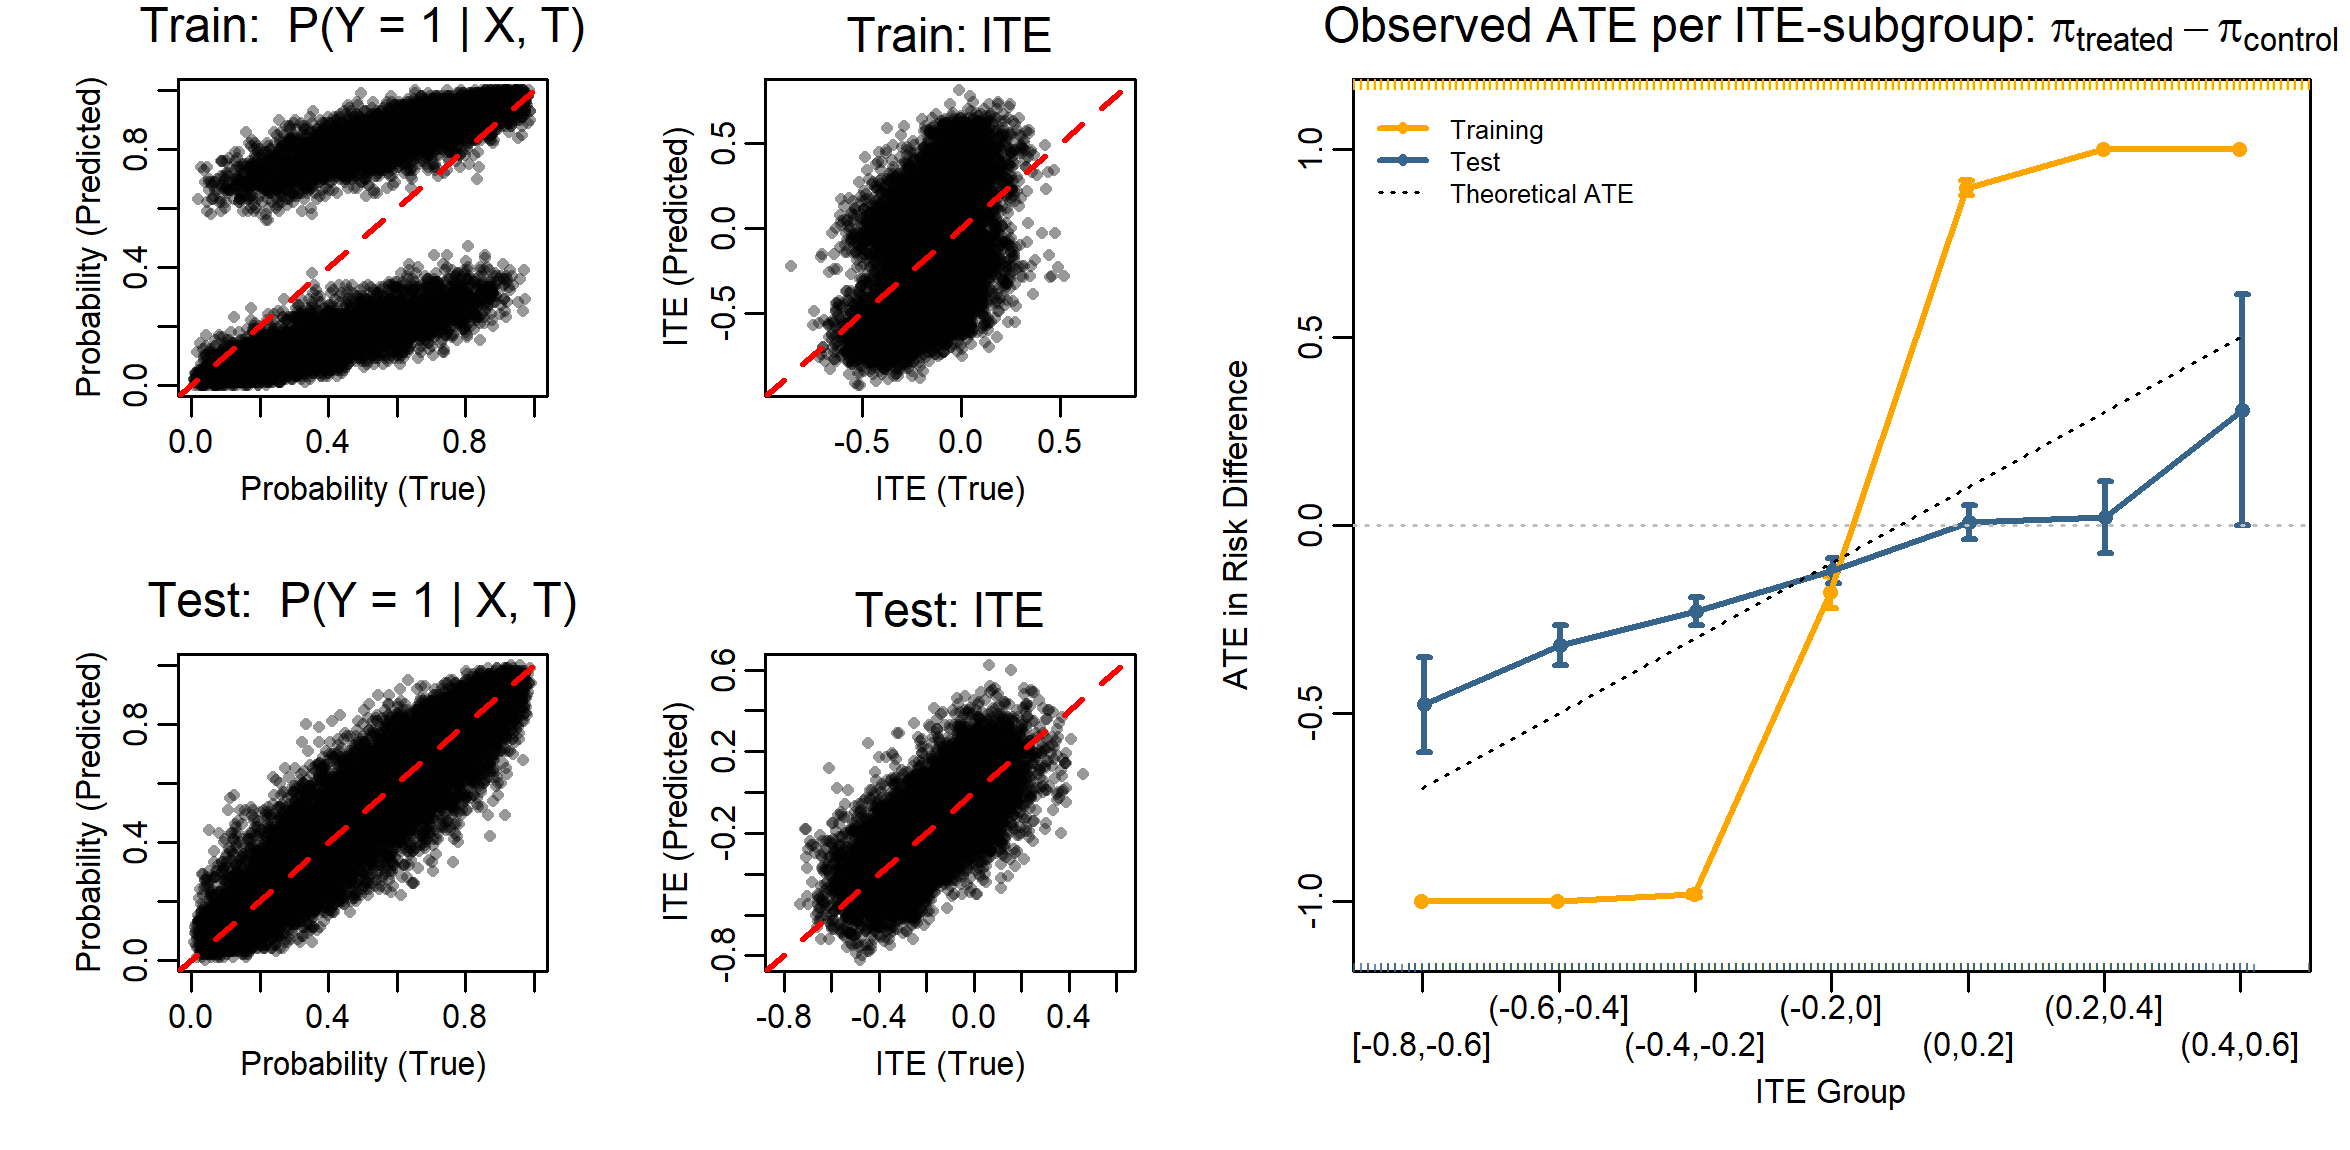
\includegraphics[width=0.9\textwidth]{img/results_ITE_simulation/fully_observed_rf_tlearner.png}
\caption{Results of the default random forest in Scenario~(1), where the DAG is fully observed and both treatment and interaction effects are strong. Left: true vs. predicted probabilities for $\text{P}(Y = 1 \mid X, T)$; Middle: true vs. predicted ITEs; Right: observed ATE in terms of risk difference per estimated ITE subgroup.}
\label{fig:fully_observed_glm_rf}
\end{figure}




\clearpage


\section{Experiment 3: Calibration plots} \label{sec:calibration_tuned_rf}

Figure \ref{fig:calibration_tuned_rf} shows the calibration plots in terms of the predicted risks against the the observed proportions of the event for the T-learner tuned random forest in Scenario (3) with weak direct and interaction effects. This is in contrast to the prediction plots presented in Section \ref{sec:results_experiment3} where we presented the true probabilities of the event $\text{P}(Y=1 \mid X, T)$ against the predicted probabilities. It becomes apparent, that tuning the random forest model out-of-bag leads to a poor calibration on the training set, but due to improved generalization it leads to a better calibration on the test set.

\begin{figure}[htbp]
\centering
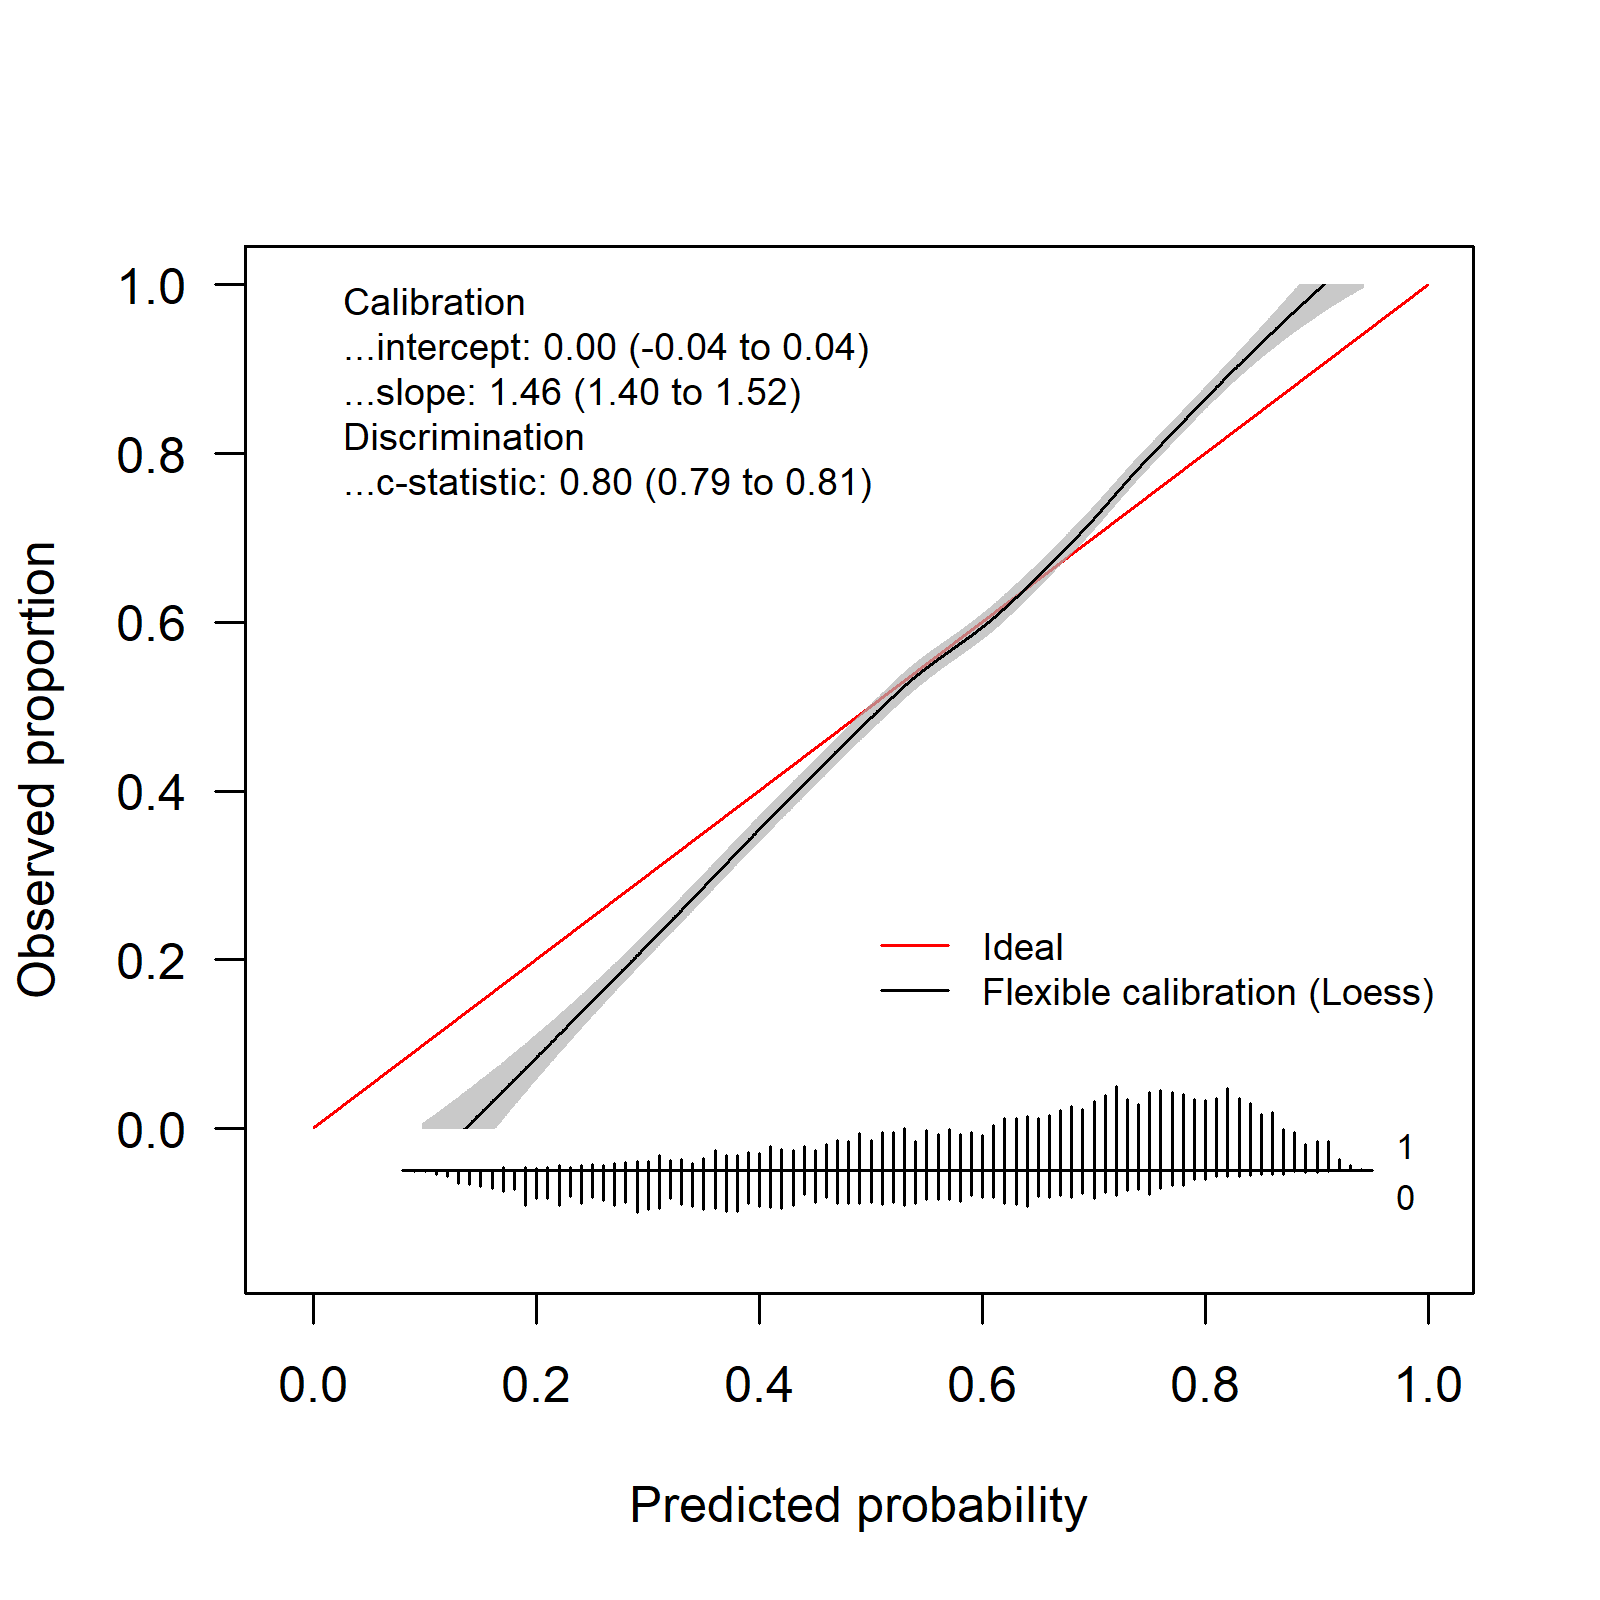
\includegraphics[width=0.45\textwidth]{img/results_ITE_simulation/small_interaction_tuned_rf_tlearnertrain_calibration_plot.png}
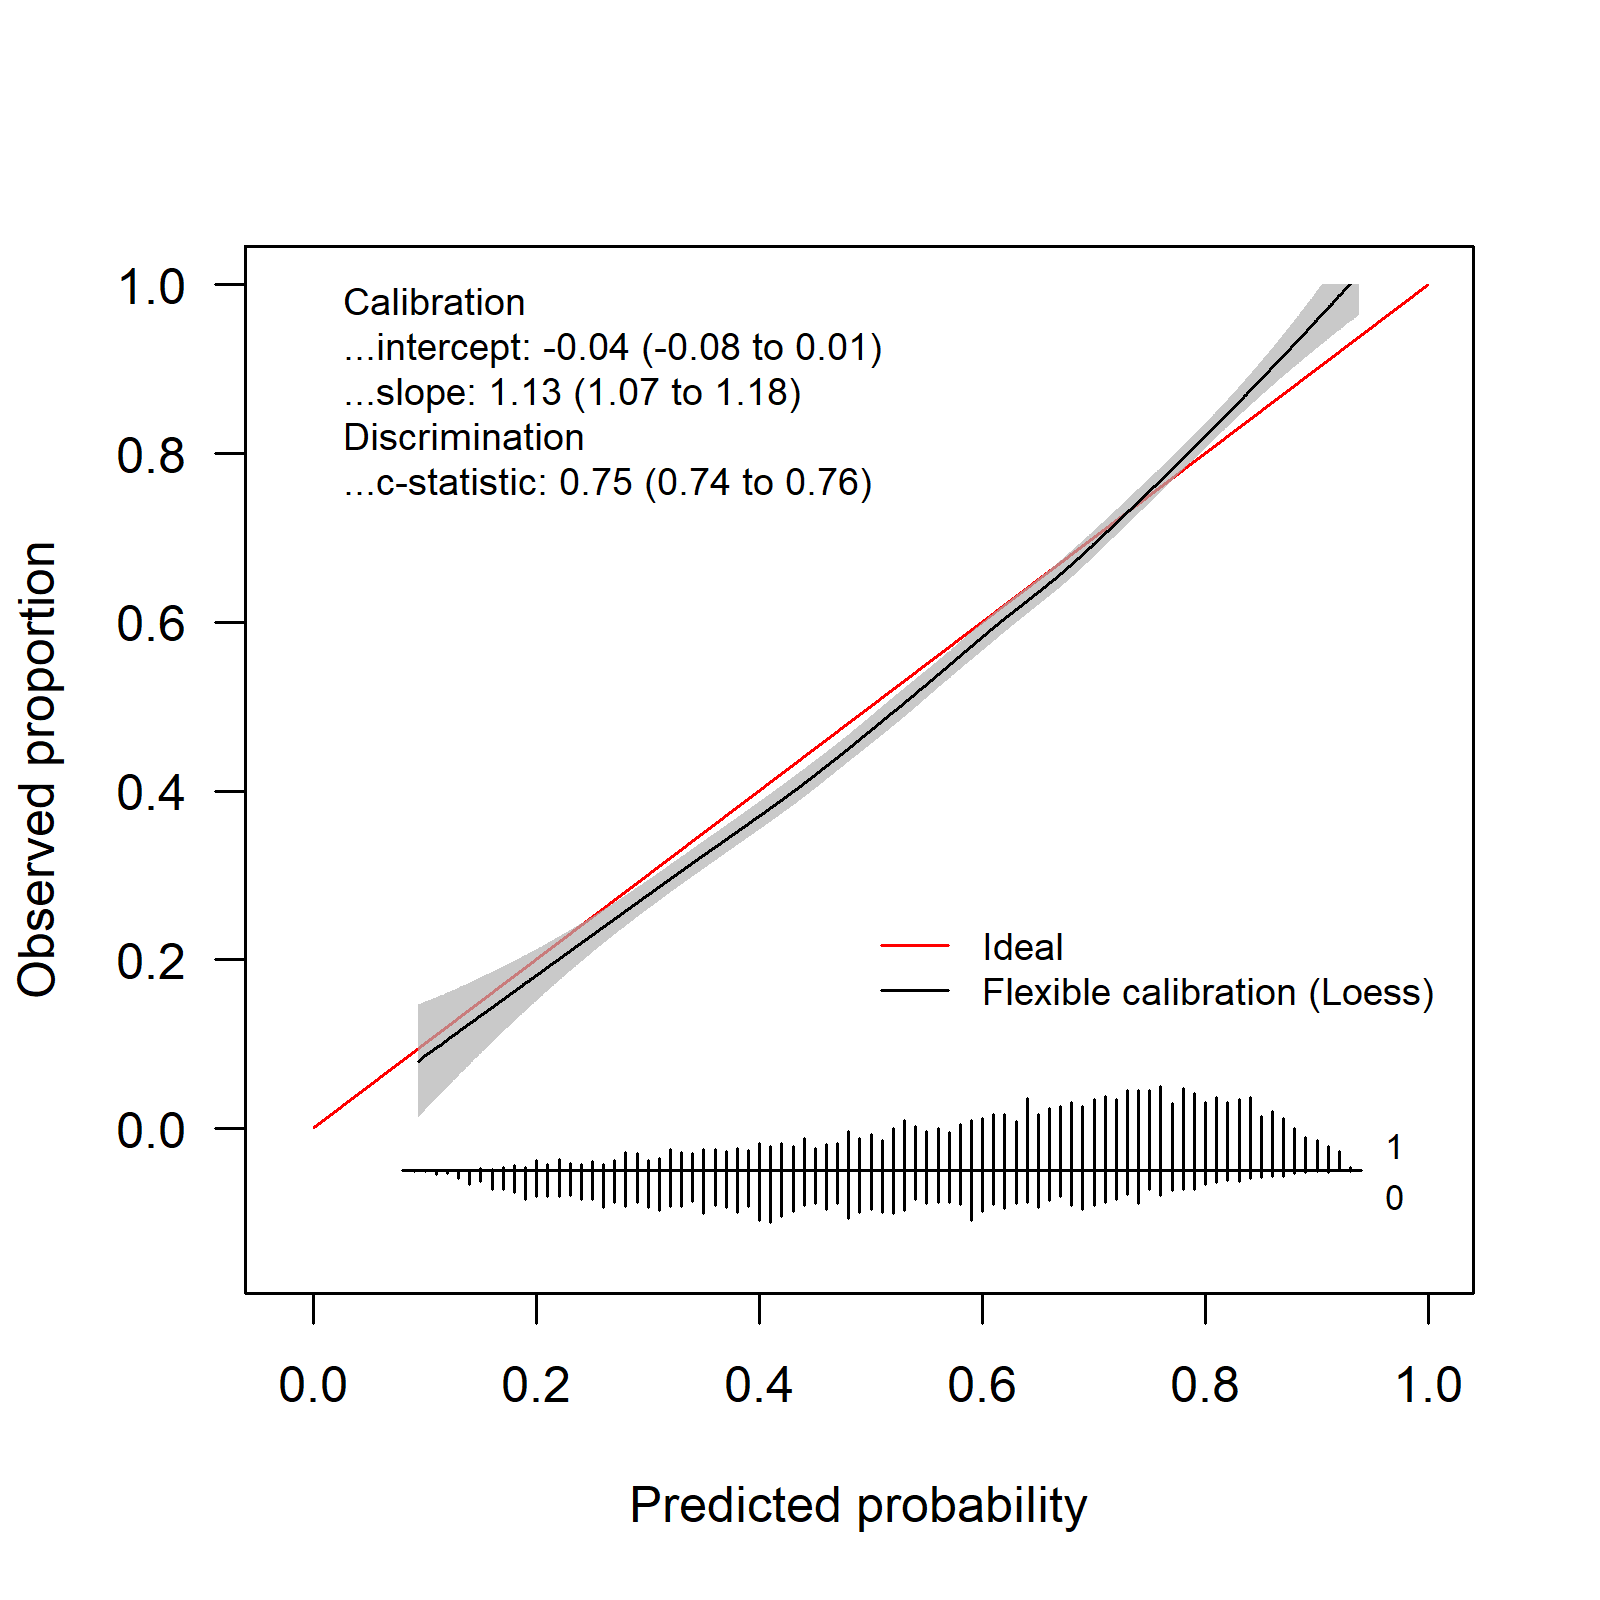
\includegraphics[width=0.45\textwidth]{img/results_ITE_simulation/small_interaction_tuned_rf_tlearnertest_calibration_plot.png}
\caption{Calibration plot for the T-learner tuned random forest for Scenario (3) with weak direct and interaction treatmetn effects. It shows the predicted risks against the the observed proportions of the event. Left: training dataset; Right: test dataset.}
\label{fig:calibration_tuned_rf}
\end{figure}


\clearpage

\section{Declaration of tools and services used} \label{sec:declaration_tools_services}

During the preparation of this thesis, I used ChatGPT, Google's Gemini and Github Copilot in order to to support language refinement, such as checking grammar, spelling and clarity of expression as well as to assist in plotting and resolving some R coding errors. After using theses tools/services, I reviewed and edited the content as needed and I take full responsibility for the content of the report.

